\documentclass{article}
\usepackage[utf8]{inputenc}
\usepackage[multiple]{footmisc}

%\usepackage{graphicx}
%\graphicspath{ {./images/} }

\usepackage{svg}
\usepackage{float}
\usepackage{amsmath} 
\usepackage{tabulary} 

\title{LUSC-A-12 LSST:UK phase A alert handling and cross match experiments}
\author{D. Morris}
\date{September 2019}

\setlength{\parskip}{1em}

%\usepackage{natbib}
%\bibliographystyle{abbrvnat}
%\setcitestyle{authoryear,open={((},close={))}}

\usepackage{breakurl}

\usepackage[style=numeric]{biblatex}
\addbibresource{references.bib}

\usepackage{xspace}
% Standard terms used throughout the document,
% defined as macro commands to maintain consistency
\newcommand{\json} {JSON\xspace}
\newcommand{\yaml} {YAML\xspace}
\newcommand{\avro} {Avro\xspace}
\newcommand{\fits} {FITS\xspace}
\newcommand{\png} {PNG\xspace}
\newcommand{\jpeg} {JPEG\xspace}
\newcommand{\parquet} {Parquet\xspace}
\newcommand{\votable} {VOTable\xspace}
\newcommand{\voevent} {VOEvent\xspace}

\newcommand{\ansible} {Ansible\xspace}
\newcommand{\docker} {Docker\xspace}
\newcommand{\dockercompose} {docker-compose\xspace}

\newcommand{\openstack} {OpenStack\xspace}
\newcommand{\dnsmasq} {\texttt{dnsmasq}\xspace}
\newcommand{\dns} {DNS\xspace}
\newcommand{\dhcp} {DCHP\xspace}

\newcommand{\ischnura} {Ischnura\xspace}
\newcommand{\esperia} {Esperia\xspace}
\newcommand{\enteucha} {Enteucha\xspace}

\newcommand{\libvirt} {\texttt{libvirt}\xspace}
\newcommand{\cloudinit} {\texttt{cloud-init}\xspace}
\newcommand{\kickstart} {kickstart\xspace}
\newcommand{\sysadmin} {system-admin\xspace}
\newcommand{\stevedore} {\textit{Stevedore}\xspace}

\newcommand{\btrfs} {\texttt{btrfs}\xspace}
\newcommand{\filesystem} {file-system\xspace}
\newcommand{\scaleable} {scaleable\xspace}

\newcommand{\paas} {PaaS\xspace}
\newcommand{\datacenter} {datacenter\xspace}
\newcommand{\webservice} {webservice\xspace}

\newcommand{\redhat} {RedHat\xspace}
\newcommand{\fedora} {Fedora\xspace}

\newcommand{\github} {GitHub\xspace}

\newcommand{\kafka} {Kafka\xspace}
\newcommand{\flink} {Flink\xspace}
\newcommand{\spark} {Spark\xspace}
\newcommand{\cassandra} {Cassandra\xspace}
\newcommand{\zookeeper} {Zookeeper\xspace}

\newcommand{\kftopic} {\textit{topic}\xspace}
\newcommand{\kftopics} {\textit{topics}\xspace}
\newcommand{\kfstream} {\textit{stream}\xspace}
\newcommand{\kfstreams} {\textit{streams}\xspace}
\newcommand{\kfbroker} {\textit{broker}\xspace}
\newcommand{\kfbrokers} {\textit{brokers}\xspace}
\newcommand{\kfconsumer} {\textit{consumer}\xspace}
\newcommand{\kfconsumers} {\textit{consumers}\xspace}
\newcommand{\kfproducer} {\textit{producer}\xspace}
\newcommand{\kfproducers} {\textit{producers}\xspace}
\newcommand{\kfpublisher} {\textit{publisher}\xspace}
\newcommand{\kfpublishers} {\textit{publishers}\xspace}
\newcommand{\kfsubscriber} {\textit{subscriber}\xspace}
\newcommand{\kfsubscribers} {\textit{subscribers}\xspace}

\newcommand{\apache} {Apache\xspace}
\newcommand{\confluent} {Confluent\xspace}

\newcommand{\kubernetes} {Kubernetes\xspace}
\newcommand{\virtualbox} {VirtualBox\xspace}
\newcommand{\vagrant} {Vagrant\xspace}
\newcommand{\kvm} {KVM\xspace}
\newcommand{\vlan} {VLAN\xspace}

\newcommand{\fifo} {FIFO\xspace}
\newcommand{\junit} {JUnit\xspace}

\newcommand{\mariadb} {MariaDB\xspace}
\newcommand{\hsqldb} {HSQLDB\xspace}
\newcommand{\cqengine} {CQEngine\xspace}
\newcommand{\crossmatch} {crossmatch\xspace}

\newcommand{\mirrormaker} {Mirror Maker\xspace}
\newcommand{\schemaregistry} {Schema Registry\xspace}

\newcommand{\serz}      {serialize\xspace}
\newcommand{\serzed}    {serialized\xspace}
\newcommand{\serzer}    {serializer\xspace}
\newcommand{\serzers}   {serializers\xspace}
\newcommand{\deserz}    {deserialize\xspace}
\newcommand{\deserzed}  {deserialized\xspace}
\newcommand{\deserzer}  {deserializer\xspace}
\newcommand{\deserzers} {deserializers\xspace}
\newcommand{\deserzing} {deserializing\xspace}

\newcommand{\phasea} {phase A\xspace}
\newcommand{\phaseb} {phase B\xspace}
\newcommand{\stageone} {stage-1\xspace}
\newcommand{\stagetwo} {stage-2\xspace}
\newcommand{\stagethr} {stage-3\xspace}

\newcommand{\ztf} {ZTF\xspace}
\newcommand{\lsst} {LSST\xspace}
\newcommand{\lsstuk} {LSST:UK\xspace}
\newcommand{\lasair} {Lasair\xspace}

\newcommand{\gaia} {Gaia\xspace}
\newcommand{\cunine} {CU9\xspace}

\newcommand{\cam} {Cambridge\xspace}
\newcommand{\ral} {RAL\xspace}
\newcommand{\roe} {ROE\xspace}
\newcommand{\wfau} {WFAU\xspace}
\newcommand{\iris} {IRIS\xspace}
\newcommand{\uedin} {University of Edinburgh\xspace}
\newcommand{\testplatform} {test platform\xspace}

\newcommand{\eleanor} {Eleanor\xspace}
\newcommand{\cumulus} {Cumulus\xspace}

\newcommand{\hdisk} {disk\xspace}

\newcommand{\footurl}[1] {\footnote{\burl{#1}}}

\usepackage{color}
\usepackage{listings}
\usepackage{changepage}

\usepackage{courier}
%\usepackage{beramono}


\lstset{basicstyle=\ttfamily\small}
\lstset{basewidth={0.5em,0.5em}}

\definecolor{codeblue}{RGB}{42,0,255}
\definecolor{codegreen}{RGB}{63,127,95}
\definecolor{codelilac}{RGB}{127,0,85}

\lstloadlanguages{Java}
\lstdefinestyle{Java}{
    language=Java,
    identifierstyle=\color{codeblue},
    commentstyle=\color{codegreen}\textit,
    keywordstyle=\color{codelilac},
    keepspaces=true,
    morekeywords={enum},
    }

\newcommand{\javaname}[1] {{\ttfamily\color{codeblue} #1}}
\newcommand{\javaplural}[1] {\javaname{#1}s}

\lstloadlanguages{SQL}
\lstdefinestyle{SQL}{
    language=SQL,
    commentstyle=\color{codegreen}\textit,
    keepspaces=true,
    keywordstyle=\color{codeblue},
    morekeywords={enum},
    }

% YAML formatting.
% https://tex.stackexchange.com/questions/152829/how-can-i-highlight-yaml-code-in-a-pretty-way-with-listings

% \usepackage[dvipsnames]{xcolor}
\newcommand\YAMLcolonstyle{\ttfamily\small\color{codeblue}}
\newcommand\YAMLkeystyle{\ttfamily\small\color{codeblue}}
\newcommand\YAMLvaluestyle{\ttfamily\small\color{codegreen}}

\makeatletter
% here is a macro expanding to the name of the language
% (handy if you decide to change it further down the road)
\newcommand\language@yaml{yaml}

\expandafter\expandafter\expandafter\lstdefinelanguage
\expandafter{\language@yaml}{
    keywords={true,false,null,y,n},
    keywordstyle=\color{codeblue},
    basicstyle=\YAMLkeystyle, % assuming a key comes first
    sensitive=false,
    comment=[l]{\#},
    morecomment=[s]{/*}{*/},
    commentstyle=\color{codegreen}\textit,
    stringstyle=\color{codegreen}\textit,
    moredelim=[l][\color{orange}]{\&},
    moredelim=[l][\color{magenta}]{*},
    moredelim=**[il][\YAMLcolonstyle{:}\YAMLvaluestyle]{:}, % switch to value style at :
    morestring=[b]',
    morestring=[b]",
    literate =  {---}{{\ProcessThreeDashes}}3
                {>}{{\textcolor{red}\textgreater}}1     
                {|}{{\textcolor{red}\textbar}}1 
                {\ -\ }{{\mdseries\ -\ }}3,
}

% switch to key style at EOL
\lst@AddToHook{EveryLine}{\ifx\lst@language\language@yaml\YAMLkeystyle\fi}
\makeatother
\newcommand\ProcessThreeDashes{\llap{\color{codegreen}\mdseries-{-}-}}

\begin{document}

\maketitle

%TODO Citeable DOI GitHub repositories.
%https://academia.stackexchange.com/a/20999
%https://github.blog/2014-05-14-improving-github-for-science/
%https://guides.github.com/activities/citable-code/

\tableofcontents
\clearpage

\section{Introduction}
\label{introduction}
This document describes some experiments designed to address some of the challenges we expect to encounter implementing a scalable architecture for a real-time alert processing system for the \lsstuk\footurl{https://www.lsst.ac.uk/} project capable of handling the data rates expected during the lifetime of the \lsst\footurl{https://www.lsst.org/} project.

The design criteria for the system include the following requirements:
\begin{itemize}
  \item Capable of meeting the initial expected data rate from the \lsst project.
  \item The ability to increase the processing speed of the system by adding new resources.
  \item The ability to increase the storage capacity of the system by adding new resources.
  \item Minimising the downtime required to add new resources to the system.
  \item The resilience of the system to individual component failures.
\end{itemize}

Additional criteria set by the requirements of the \lsstuk project and the planned deployment on resources provided by the \iris eInfrastructure initiative\footurl{https://www.iris.ac.uk/}:
\begin{itemize}
  \item It should be possible to implement the system using standard hardware resources.
  \item It should be possible to deploy the system on generic cloud compute resources.
\end{itemize}

The target data rates for the experiments are:
\begin{itemize}
  \item Sustained 1,000 alerts per second
  \item Stretch goal 10,000 alerts per second
\end{itemize}

These numbers are based on the values given in table 29 of the \lsst System Science Requirements Document (LPM-17)\footurl{https://docushare.lsst.org/docushare/dsweb/Get/LPM-17}.

\begin{quote}
\textit{“Specification: The system should be capable of reporting such data for at least transN candidate transients per field of view and visit”}
\end{quote}

\begin{center}
\begin{tabular}{|l|l|l|l|}
\hline
\textit{Quantity} & \textit{DesignSpec} & \textit{MinimumSpec} & \textit{StretchGoal} \\ \hline
\textit{transN}   & $10^{4}$            & $10^{3}$             & $10^{5}$             \\ \hline
\end{tabular}
\end{center}

The \textit{transN} value sets the number of alerts per visit, this combined with the expected cadence of 30 seconds per visit gives us our target evaluation criteria of 1,000 alerts per second and the stretch goal of 10,000 alerts per second for these experiment.

To meet the scalability and fault tolerance requirements we developed a micro-service\footurl{https://microservices.io/} based design for the alert processing system, where multiple instances of each component can be deployed in parallel, using \kafka\footurl{https://kafka.apache.org/} to distribute the alerts between components in the pipeline.

Our initial reason for selecting \kafka as the message transport technology was informed by the work done by M. Patterson\cite{Patterson_2018} and colleagues developing the alert processing infrastructure for the Zwicky Transient Facility (ZTF)\footurl{https://www.ztf.caltech.edu/} project.

The \ztf alert processing infrastructure is considered a prototype for the \lsst alert processing infrastructure, which is planning to use a similar \kafka based system as the primary distribution protocol for the \lsst level 1 alert stream.

Our initial introduction to \kafka was as the external site to site delivery protocol for the \ztf and \lsst alert streams. 

However, \kafka was originally designed as an internal message delivery system for data streams processing applications within a data center, rather than an external site to site delivery system.

As we learned more about \kafka and its capabilities it became clear that it would be an ideal technology for implementing the internal data streams linking together the individual micro-service components within the system, enabling us to build a flexible and \scaleable system.


\section{High level outline}
\label{high-level-outline}

The proposed architecture design consists of three layers of components, connected together by \kafka streams.

\subsection{Stage 1, input buffer}
\label{stage-1}

The first stage of the system architecture is a local \kafka mirror configured as a 7 day first-in first-out (\fifo) buffer of the live stream from \lsst. This buffer has a number of functions:

\subsubsection{Local endpoint}
\label{stage-1.local-endpoint}
Access to the upstream \kafka endpoint provided by \lsst is bandwidth limited, and will be limited to a small group of clients who are allowed to connect. Even if these restrictions are relaxed it will still make sense for each project to only make one connection to the upstream service.
This is particularly relevant in our case, as our connection to the upstream service involves a trans-Atlantic connection.
Implementing a mirror of the upstream service will provide a local \kafka endpoint for our other components to connect to, enabling multiple components to connect to the primary input \kafka stream without placing an unnecessary load on our external network connection or the upstream service.

\subsubsection{Local buffer}
\label{stage-1.local-buffer}
Configuring our mirror of the upstream service as a 7 day \fifo buffer, makes our system more resilient to networking issues and component failures.
If a component in our system fails, the 7 day buffer gives us time to fix the issue, test and restart the failed component using data from our local buffer.

\subsubsection{Partition count}
\label{stage-1.partition-count}
The number of partitions in a \kafka stream puts an upper limit on the level of parallelism that downstream components can apply to processing a stream (see section \ref{kafka-partitions}).
Deploying a buffer at the input to our system give us direct control over the number of partitions available to the rest of our processing components.

\subsubsection{Schema mapping}
\label{stage-1.schema-mapping}
The ZTF and LSST alert messages are encoded using the \apache\avro\footurl{https://avro.apache.org/} binary encoding format. 

In addition to the binary message content, the current live stream from \ztf uses an inline schema to describe the message schema. Every message carries a copy of its schema embedded in the message header \serzed as a plain text \json\footurl{https://www.json.org/} document.
This means the alert messages are self-describing, and provides some insulation from side effects of schema changes for clients.
However, embedding the schema in every message adds a non-trivial overhead, particularly if the stream only contains a small number of well known message types.

Our understanding is that the \lsst project intend to use a service like the \schemaregistry\footurl{https://www.confluent.io/confluent-schema-registry/} to manage their \avro schema, and each message will only include a schema identifier rather than the full schema. This reduces the overhead associated with using an inline schema to describe the messages. However, the schema identifier will be specific to the upstream project's \schemaregistry. This means we will need to provide a mapping from their schema identifiers to the corresponding schema identifiers in our own local \schemaregistry.
This translation can be handled by the input buffer, replacing the upstream schema identifier with the the corresponding local identifier as it receives the messages.

\subsubsection{Topic merge}
\label{stage-1.topic-merge}
The current stream from \ztf is published as a series of separate daily \kftopics, one for each night of observations. Handling the data in chunks like this a useful format to manage the bulk transfer and archiving of the data. When making backups or managing data transfers it is convenient to be able to refer to [\textit{the data from yesterday}] or [\textit{the data from three days ago}]. However, our end users are more likely to want to access [\textit{the live data from \lsst}], in one continuous stream.

Ideally it would be useful to have access to both a single continuous \kfstream for the science use cases, and a series of separate daily \kftopics for system administration and backups.

Depending on how the live data stream from \lsst is configured, as a single continuous \kfstream or as separate daily \kfstreams, our \fifo buffer can either split the continuous \kfstream into separate \kftopics for the system administration tasks, or merge the separate \kftopics into one continuous \kfstream for our science uses.

By placing our own \fifo buffer at the head of our processing chain we are insulated from changes to the design of the upstream \kfstream from \lsst.
Our \fifo buffer would handle changes to the \kftopics and schema by the upstream service and present a consistent set of \kftopics and schema to our internal components.

\subsubsection{Test data}
\label{stage-1.test-data}
The same \kafka service can also provide access to a set of test data that will be useful for our own integration testing, and for end users developing and testing their own custom processors.

Example test data:
\begin{itemize}
  \item Known sets of simulated data for specific scenarios.
  \item Known subsets of historical data from \ztf.
  \item \ztf data with static, inline and registered schema.
  \item \lsst data with static, inline and registered schema.
\end{itemize}

The advantage of using the same \kafka service to store and serve test data is it means our components can use the same libraries and configuration tools in development, testing and live production.

In order to evaluate this use case we have been experimenting with maintaining a \kafka \kfbroker configured as a rolling 7 day \fifo buffer, using it as source for test data and as a permanent data archive.
In the process we have learned a lot about configuring and administering a \kafka \kfbroker, which we describe in more detail in Section \ref{kafka-compendium}.
The key points are :
\begin{itemize}
    \item Deploying \kafka as a 7 day \fifo buffer requires very little additional configuration. The default out of the box configuration deploys a simple \fifo buffer.
    \item Having access to a set of test data is extremely useful for developing processing components. However, if the tests are intended to gather performance statistics, then care is needed to coordinate the tests and isolate them from each other.
    \item It is possible to configure \kafka as a long term data archive. However, we encountered some issues to do with managing the service and maintaining the data which would suggest that \kafka is probably not the best tool for this. 
\end{itemize}

To date these experiments have been using the standard \mirrormaker\footurl{https://cwiki.apache.org/confluence/pages/viewpage.action?pageId=27846330} service from the \apache \kafka project.
In order to provide the additional functionality such as topic merging and schema translation we would need to develop our own implementation of the \mirrormaker service.
Based on our experience of working with the tools and client libraries provided by the \apache \kafka project this should be relatively easy to implement.

\subsection{Stage 2, workflow components}
\label{stage-2}
The second stage of processing consists of a set of loosely coupled components that consume data from a \kfstream, apply a filter or processing step, and produce a new stream of results.

\kafka is designed to distribute messages to multiple clients reading messages from the same \kfstream at different speeds. Section \ref{kafka-offsets} describes how \kafka supports this in more detail, but what it means for us is we can have multiple different components subscribed to the output of the \stageone buffer processing the messages at different rates without interfering with each other.

A mixture of slow, low bandwidth, components gradually working through the alert messages can subscribe to the same \kafka \kfstream as high speed, high bandwidth, components processing the alert messages as fast as possible. The \kafka service takes care of buffering the data so that all of the components get to see all of the alert messages in the right order.

\subsubsection{High speed components}
\label{stage-2.high-speed.components}

Some example high speed processors might include :
\begin{itemize}
  \item \crossmatch alert messages with a watch list and trigger actions.
  \item \crossmatch alert messages with archive catalogs and generate annotated results.
\end{itemize}

These examples are considered high speed components is because their output will be used as the input for other components, creating a pipeline or workflow.
They must be able to process the incoming data as fast as it is arriving, producing their results with the minimum latency between input and output.
In order to meet these requirements, these components are designed to be able to run multiple instances in parallel, increasing the data throughput by processing multiple alert messages at a time.

Some example medium speed components might include :
\begin{itemize}
  \item Read alert messages and write candidates to \cassandra database.
  \item Read alert messages and write candidates to \mariadb database.
\end{itemize}

These examples are considered medium speed components because the performance of the database they are writing to will be a limiting factor in determining the maximum data rate they can handle. A key factor in the performance of these components will depend on whether the database platform they are using is able to handle multiple writes in parallel.

%As part of our work for \phasea of the \lsstuk project we have performed some initial experiments looking at %the performance achievable writing alert message candidates to a \cassandra database. The results of these %tests are described in more detail in section \ref{cassandra-writer}.

\subsubsection{Low speed processors}
\label{stage-2.low-speed.processors}

Some example low speed components might include :
\begin{itemize}
  \item Read alert messages and write them to \avro files for backup.
  \item Read alert messages and write candidates to \parquet files for downstream \spark analysis.
  \item Read alert messages, extract the light curves and write them to \fits or \votable files for downstream analysis.
  \item Read alert messages, extract the images and write them to FITS/PNG/JPEG files for downstream display or analysis.
\end{itemize}

These examples are considered low speed processors because there is no science case requirement for them to produce results at high speed. Depending on the amount of data processing required by their algorithm they can operate with a small number of concurrent processes.

However, they will still need to be able to meet a minimum level of processing speed in order to process a days worth of data within a day. Based on our experience with \ztf the input data rate is likely to be non-uniform, periods with a very high rate of alerts, and periods with a much lower rate, and the daily totals can vary by several orders of magnitude (from 100 to 1,000,000 alerts per night).
While the low speed components don't need to be able to match the peak bandwidth of the busy periods, they do need to be able to process the cumulative data from each night fast enough to have completed that night's worth of data before the next night's data begins.

\subsubsection{Component libraries}
\label{stage-2.component-libraries}

In order to help develop these processors and filters the \lsstuk project should provide a set of Java and Python libraries that implement the support functionality needed to connect to \kafka services, subscribe to \kftopics, read and write messages, \serz and \deserz \avro messages etc.

Using a common set of well tested libraries will help to make our own components easier to develop and more reliable to use. It will also help to lower the barrier to entry for 3rd party developers to create their own processors and filters.

In order to support the \crossmatch tests described in Section \ref{crossmatch-algorithms} we developed a set of Java classes and interfaces that prototype this architecture.
We also looked at automating the deployment of the components using a common \yaml configuration file syntax that enables non-programmers to connect together stream processing components to build a workflow.

Further details of the Java API and a proposed configuration schema are given in sections \ref{component-libraries.java-interfaces} and \ref{workflow-configuration}.

\subsection{Stage 3, Spark analysis}
\label{stage-3}

Part of our work for \phasea involved background research into a number of different analysis platforms in use in the data analytics field and some of the capabilities provided by the different software platforms available.

Based on the results of our research, we expect that it may be possible to meet a significant portion of our science use cases using something like the Spark Structured Streaming \footurl{https://spark.apache.org/docs/latest/structured-streaming-programming-guide.html} or \apache\flink\footurl{https://flink.apache.org/}  processing engines coupled with filtered streams produced by the \stagetwo processing components.

%\section{Phase-A experiments}
%\label{experiments}
%
%As part of our work for \phasea of the \lsstuk project we performed a number of experiments that looked a %specific parts of the design outlined in the previous sections.

\section{Deployment platforms}
\label{deployment-platforms}

The software components developed for the \phasea experiments were deployed twice, once on a set of physical machines at ROE, and again on an \openstack\footurl{https://www.openstack.org/} platform provided by the \uedin IT services.

Using the different systems helped us to learn how to manage service deployments, to evaluate the costs and benefits of the different platforms, and learn how suitable they would be for deploying live production services.

\subsection{\eleanor \openstack}
\label{deployment-eleanor.openstack}

The first set of \kafka deployments for the \phasea  experiments were deployed on the \eleanor\footurl{https://www.ed.ac.uk/information-services/computing/computing-infrastructure/cloud-computing-service/researcher-cloud-service-eleanor}  \openstack platform provided by \uedin IT services.

To support this deployment we developed set of shell script tools for managing virtual machines on the \eleanor \openstack system. 
The tools were packaged in a \docker container that included the \openstack command line client along with a set of shell scripts that helped to manage virtual machines and some parser utilities that make it easier to handle the \eleanor-specific syntax for things like virtual machine flavors and the internal and external network addresses.

These \docker containers formed the basis for a set of toolkit containers containing client tools for \libvirt, \openstack and \ansible\footurl{https://www.ansible.com/} which have since been published as a separate project on \github\footurl{https://github.com/wfau/atolmis}.

The experiments deployed on the \eleanor system explored a number of different \kafka configurations including a long term archive and a rolling 7 day FIFO buffer.

During this work we discovered and solved a number of minor issues involved with administering \kafka deployments. Many of these were simply discovering easy-to-make mistakes, learning how to identify them, and figuring out good practice rules for avoiding them.

Some of the key lessons learned were:
\begin{itemize}
    \item Configuring \kafka as a \fifo buffer is close to the default 'out of the box` configuration.
    \item Configuring \kafka as a long term archive is possible, but there are issues regarding data management that mean it is probably not the best solution (this is discussed in more detail in Section \ref{kafka-archive}). 
    \item A \kafka instance will fail fast. If there is anything wrong with the service or its configuration, e.g. out of \hdisk space in a log directory, it will disconnect itself from the \kafka cluster and shut itself down.
    \item The host names or IP addresses used for the \kafka server endpoint addresses need to be resolvable and accessible from both inside and outside the \openstack system, which can cause problems at the network routing level when using \docker containers inside \openstack (see Section \ref{kafka-hostnames} for more details).
\end{itemize}

Mid way through the series of \phasea experiments on \kafka the \eleanor system experienced a number of issues to do with the configuration of the \openstack network components which eventually lead to the platform being shutdown.
An unintended side effect of this was that we gained experience in trying to maintain a \kafka service on an unstable platform, and learned some important insights into the stability and resilience issues inherent in deploying services on a cloud compute infrastructure.

\subsection{Testbed platform}
\label{deployment-testbed.platform}

As part of our work for \phasea we were involved in specifying and configuring some of the hardware for the \lsstuk \testplatform installed at \roe.

Over the duration of the \phasea work the \testplatform has grown from an initial set of two machines to six machines for the \lsstuk project and two machines for the \gaia \cunine project deployed in the same \datacenter at \roe (with to more expected early in 2020). Setting up a full \openstack deployment for just the two machines available at the start of \phasea did not justify the cost in time and resources it would involve. In fact with just two machines available the \openstack services themselves would have take up a significant portion of the available resources leaving little space left for running the tests.

As a result the development of the \testplatform started with a basic deployment of \libvirt\footurl{https://libvirt.org/} and added layers of tools as and when they were required.

Another reason for not using \openstack to provision resources on the \testplatform is that one of the things we wanted to explore with the local \testplatform is how different configurations of software and hardware effected the system performance. To do this we needed direct control over how and where the resources were allocated and direct access to the underlying system to be able to monitor the performance. 

Given that we now have access to at three different \openstack systems, the \eleanor system managed by \uedin IT services and the \iris systems at \ral and \cam, it made sense to keep the \testplatform for low level experiments with direct access to the physical hardware rather than adding the additional abstraction layers of an \openstack deployment.

\subsection{\ischnura \libvirt}
\label{deployment.ischnura-libvirt}

The current configuration (Q3 2019) of the \testplatform uses a set of command line tools available from the \ischnura project\footurl{https://github.com/Zarquan/ischnura} on \github
to provision virtual machines on the worker nodes.

The \ischnura tools provide a simple cookie-cutter tool for creating identical virtual machines as quickly as possible.
However the \ischnura tools only supported basic \libvirt deployments with the user account and ssh keys hard coded into the virtual machine images.
In order to support deployments on the \eleanor platform using the same virtual machine images we modified the \ischnura tools to use the same \cloudinit\footurl{https://cloud-init.io/} process that is used by \openstack to configure user accounts and ssh keys in new virtual machines.

This work involved modifying the \ischnura tools to write the details of the admin user account to a \cloudinit configuration file on the host system, wrap the directory containing the configuration file as an ISO9660\footurl{https://en.wikipedia.org/wiki/ISO_9660} image, and mount that as a CDROM device on the new virtual machine. During the boot process the \cloudinit software will check a number of different options for configuration information, including a standard location on the local network or local CDROM device. If it does find \cloudinit configuration data it will use the metadata to configure the admin account, including the list of ssh \texttt{authorized\_keys} and the \texttt{sudo} permissions.

As a result of this work the administrator account in a new virtual machine will be automatically initialized  with the correct user account and ssh keys whether created using the \ischnura on the \testplatform, at \roe, the \eleanor \openstack system at the \uedin or an \openstack system provided by \iris.

\subsection{Network configuration}
\label{deployment-testbed.network-layers}

The network configuration for the \testplatform has evolved over the period of the \phasea project as the test requirements changed and the number of physical machines grew. 

The initial deployment used the default NAT\footurl{https://en.wikipedia.org/wiki/Network_address_translation} based networking available as part of a standard \libvirt deployment. This works for local services deployed on virtual machines running on the same physical host. As soon as we needed to have components running on different physical hosts we needed to replace this with a network capable of spanning multiple physical machines.

The first iteration of this was to use a \textit{'routed'} network configuration that still used the local \dnsmasq\footurl{http://www.thekelleys.org.uk/dnsmasq/doc.html} service provided by the \libvirt service on each of the physical machines, but configured the \libvirt network to act as a router, making the the virtual machines accessible on the wider network.
To enable name resolution between virtual machines the full set of IP addresses and host names were added to the \texttt{/etc/hosts} file on each physical machine, 
This was sufficient to enable services and clients on different virtual machines to connect to each other, as long as the physical hosts are connected to the same physical network segment.
This is quick and easy to set up for a small number of physical machines, but becomes progressively more complex to administer as the number of machines increases.
In theory it would be possible to automate the configuration of this using a deployment tool such as \ansible. However, beyond about two or three physical hosts the law of diminishing returns applies and it was better to spend the resources setting up a full virtual network for the \testplatform.

The third iteration of network configuration for the \testplatform defined a virtual local area network (\vlan)\footurl{https://en.wikipedia.org/wiki/Virtual_LAN} at the level of the \datacenter network switches, which means the physical machines are connected to their own virtual network isolated from the rest of the university systems. The network interface on each physical host is configured as a bridge interface, and the \libvirt network layer is configured to connect network interfaces on the virtual machines directly to the bridge interface on their host. The result is that all of the physical and virtual machines are connected to the same local network, and everyone can 'see' and reach everyone else.

\subsection{\texttt{dnsmasq} service}
\label{deployment-testbed.dnsmasq}

Placing all of the virtual machines on the same \vlan as their physical hosts, with the \libvirt network configured as a direct connection to the bridge interface meant that we could no longer use the \dnsmasq service provided by the local \libvirt instance on each of the physical machines.
In order to provide the \dhcp\footurl{https://en.wikipedia.org/wiki/Dynamic_Host_Configuration_Protocol} and \dns\footurl{https://en.wikipedia.org/wiki/Domain_Name_System} services needed to manage the IP addresses and host names across the whole of the \vlan we developed the configuration files for a \dnsmasq service to run in a \docker container.

The \docker container deployment uses a vanilla \dnsmasq \docker container published by Storytel\footurl{https://github.com/Storytel/dnsmasq}\footurl{https://hub.docker.com/r/storytel/dnsmasq/dockerfile} and adds the configuration files needed to define a set of MAC addresses, IP addresses and hostnames for the virtual machines.

Although there is no technical requirement to allocate these addresses on a per host basis, we used a template pattern to map specific groups of addresses to the virtual machines running on each physical host.
This means it is possible to identify which virtual machine is running on which physical machine just by looking at the MAC or IP address. This is extremely useful when trying debug network issues by looking at capture logs of network traffic.

The \dnsmasq \docker container was originally deployed on one of the \testplatform worker nodes, but it has since been moved to a separate physical machine allocated specifically for this purpose.
Deploying the \dnsmasq service in a \docker container made this transition much easier, and paid back the original investment in time used to set up the \docker deployment.
Once the \dnsmasq was moved off the worker node, it means all of the \testplatform worker nodes are configured as vanilla \libvirt hosts with no unique configuration or services on any of them.
 
Source code and notes for the network configuration are published in the \esperia \github project\footurl{https://github.com/wfau/esperia}.

\subsection{Ansible deployment}
\label{deployment-testbed.ansible}

The next stage of work on the \testplatform will be to develop the configuration and deployment scripts into a set of \ansible playbooks that automate the process of configuring the \dnsmasq service and deploying \libvirt and \ischnura on the worker nodes.

At the time of writing (Q4 2019) much of the configuration and deployment scripts in the \esperia project have been replaced by \ansible playbooks.
The \ansible playbooks have been extended to include setting the user accounts, ssh \texttt{authorized\_keys} and the \texttt{sudo} permissions on the physical machines. However configuring the primary network interfaces on the physical machines has not yet been implemented as an \ansible playbook. This is partly due to the chicken and egg problem inherent in trying to configure the primary network interfaces using a tool that needs a working network and ssh access to configure the target machines.

The eventual aim is to have all of the system configuration automated as \ansible playbooks, enabling the \testplatform machines to be configured for other experiments and then wiped and re-configured back to the \testplatform settings automatically.

Combining this with the work done by Li Teng\footurl{https://github.com/wfau/feipengsy} using Kayobe\footurl{https://github.com/openstack/kayobe} to deploy \openstack on hardware at \roe 
will mean we can reconfigure the \testplatform hardware to use different deployment platforms for different tests and experiments.

\subsection{Virtual machine image}
\label{deployment-vm-image}

In order to provide a reliable base for the virtual machines we have developed a standard virtual machine image for all of the tests and service deployments. Using the same base image throughout all of the experiments has a number of advantages:
\begin{itemize}
    \item Version control of the image ensures that the tests are performed under the same conditions.
    \item The same environment and tools are always available for deployment, testing and debugging.
\end{itemize}

The virtual machine image developed for the project is based on a minimal install of \redhat \fedora\footurl{https://getfedora.org/}\footurl{https://en.wikipedia.org/wiki/Fedora_(operating_system)} Linux distribution and the community edition of the \docker platform-as-a-service (\paas) tools\footurl{https://boxboat.com/2018/12/07/docker-ce-vs-docker-ee/}.

The creation of the image is automated using a \kickstart\footurl{https://en.wikipedia.org/wiki/Kickstart_(Linux)}\footurl{https://pykickstart.readthedocs.io/en/latest/kickstart-docs.html} script which is available on \github as part of the \ischnura project\footurl{https://github.com/Zarquan/ischnura/blob/master/src/kickstart/fedora-docker-base.txt}. The kickstart script starts with the base install of the operating system, adds a basic set of system administration tools and then configures the default user account, \stevedore, with permission to install and configure new software and to create and manage \docker containers inside the virtual machine.

The default user account has password access disabled, and is configured to only allow ssh access using public key authentication\footurl{https://serverpilot.io/docs/how-to-use-ssh-public-key-authentication}. However, the image itself does not contain any ssh keys. It relies on the orchestration tools to inject the correct ssh key when a virtual machine instance is created using the image as a template.
To enable this to happen, the virtual machine image is configured to use the \cloudinit tools to discover the configuration data for the instance and use it to configure the ssh keys for the user account.

\subsection{\docker \btrfs storage driver}
\label{docker.btrfs.}

Based on our earlier work using \docker \cite{Morris-2017} we opted to use a \btrfs\footurl{https://btrfs.wiki.kernel.org/index.php/Main_Page}\footurl{https://en.wikipedia.org/wiki/Btrfs} \filesystem on the virtual machines and configured the \docker service to use the \btrfs storage driver. 

Although the \btrfs \filesystem is still considered experimental by many system administrators, our own experience of using \btrfs for a number of years in a range of different applications we have found it to be both reliable and performant. In particular our experience of using it as the storage driver\footurl{https://docs.docker.com/v17.09/engine/userguide/storagedriver/btrfs-driver/} for \docker containers deployed inside virtual machines gives better results than the default \texttt{overlay2}\footurl{https://docs.docker.com/v17.09/engine/userguide/storagedriver/overlayfs-driver/#how-the-overlay2-driver-works} storage driver normally used with \docker.

\section{Crossmatch algorithms}
\label{crossmatch-algorithms}

One of the challenges the \lsstuk transient event processing will have to address is to \crossmatch the incoming event stream against archive databases of know objects. With this in mind we developed a series of experiments to compare the performance of different \crossmatch algorithms, database platforms and indexing to identify the best candidates for implementing a \crossmatch component capable of matching the live alert stream data rate from \lsst against the science catalogues held by \wfau.

The objective for these experiments is to demonstrate a \crossmatch implementation capable of meeting the target of 1,000 alerts per second set in the Introduction to this paper, and be able to scale up to meet the higher stretch goals by adding additional resources.

The experiments compared two \crossmatch algorithms, the Hierarchical Triangular Mesh (HTM)
algorithm currently used to index many of the \wfau catalogs compared with a zones based algorithm described in a 2004 Microsoft Research paper by J.Gray et al \cite{Gray-2004}.

The source code for these experiments is available in the \enteucha \footurl{https://github.com/lsst-uk/enteucha} project on \github.

\subsection{Hierarchical Triangular Mesh}
\label{crossmatch.htm}

The Hierarchical Triangular Mesh (HTM) algorithm is described in a paper by Kunszt et al. presented at the ADASS conference in 1999 \cite{Kunszt-1999} and in a subsequent paper presented at the MPA/ESO/MPE Workshop in 2000 \cite{Kunszt-2000}.

The HTM algorithm divides the celestial sphere into eight spherical triangles, and then recursively builds a quad-tree decomposing each triangle at \textit{m} into a set of 4 sub-triangles at level \textit{m+1}.

The identifier, or \textit{HTM name}, for a triangle at level \textit{n} is generated by encoding the index of the triangle within its parent \{0, 1, 2 ,3\}  as a two bit value, and concatenating this to the \textit{HTM name} of the parent triangle, \textit{n-1}, all the way up to one of the the eight top level \textit{0} triangles.

The resulting \textit{HTM name} can be used as an efficient index to identify triangles at any level in the hierarchical tree. The first two bits of the \textit{HTM name} identify the top level \textit{0} triangles, the next two bits identify the level \textit{1} triangles within the level \textit{0} parent.

Performing a \crossmatch with this algorithm involves identifying the initial triangle that contains the target position, identifying the adjacent triangles that overlap a circle centered on the target point, load the data for objects within those triangles and then compare them to see if they match our target.

The code to implement the HTM algorithm used in our tests is based on the Java library available from the SkyServer website at John Hopkins University\footurl{http://www.skyserver.org/HTM/doc/intro.aspx}\footurl{http://www.skyserver.org/htm/implementation.aspx}. However, due to licensing issues we are unable to make this part of our code open source at this time.

\subsection{Zone based algorithm}
\label{crossmatch-zones}

The zone based algorithm is described in a Technical Report MSR-TR-2004-32 by Jim Gray published by Microsoft Research in 2004 \cite{Gray-2004}.

More recently, the same zone based indexing has been used as part of the \textit{Astronomy eXtensions for Spark (AXS)} toolkit for the \apache \spark platform, described in a 2019 paper by Petar Zečević et al \cite{Zecevic-2019}.

The zone based algorithm uses a much simpler method of dividing the celestial sphere into thin horizontal zones based simply on the declination.

\begin{lstlisting}[]
    zoneNumber = floor((dec+90)/zoneHeight)
\end{lstlisting}

The initial step of the zone based algorithm is much simpler to implement and faster to execute than the equivalent steps needed to locate the target triangle in the HTM algorithm, requiring only simple floating point and integer arithmetic operations compared to the complex trigonometry involved in the HTM algorithm.

The trade off is to start the selection process using very simple steps, significantly reducing the amount of data involved, and then use more complex steps later in the process.

\subsection{Database platform}
\label{database-platform}

Due to the nature of the problem, performing a \crossmatch using a conventional database system tends to be limited by physical I/O performance. The overhead of getting the data off \hdisk can obscure the relative performance of the indexing algorithms.

In order to maximize the performance, the experiments used an in-memory instance of the Hyper SQL Database (\hsqldb)\footurl{http://hsqldb.org/} database engine to evaluate the different algorithms. The reasoning behind this is that once the I/O data access bottle neck is removed from the equation, the differences between the indexing algorithms becomes much more significant.

\subsection{Data generator}
\label{test-data-generator}

The aim of the experiments was to test the algorithms with large enough data sets to show up differences in the performance of the algorithms.
A side effect of this was that loading and indexing the test data into the target systems took significantly more time than the actual test searches themselves.
In order to mitigate this as much as possible, the data generator was designed to enable us to run a set of tests, add more data to the data set and then re-run the same tests again.

The data generator was designed to add data successively larger and larger sets of points in a square grid around an initial central target point, scaling up the number of points by a power of 2 each time.
After each iteration the test data set will contain \(((2^n)+1)^2\) points.

Given an initial point at the center. The first pass of the algorithm will add eight additional points to create a 3x3 grid of points around the target. 
\begin{figure}[h]
\includesvg{images/data-count-01.svg}
\caption{$n=1 \ :\ ((2^n)+1)^2 = 3^2 = 9 \ points, 1 \ match$}
\label{fig:data-count-03}
\end{figure}

The second pass will add an additional sixteen points in between the original nine, to create a 5x5 grid of 25 points around the target. 
\begin{figure}[h]
\includesvg{images/data-count-02.svg}
\caption{$n=2 \ :\ ((2^n)+1)^2 = 5^2 = 25 \ points, 9 \ matches$}
\label{fig:data-count-03}
\end{figure}

The third pass will add a further fifty six points to create a 9x9 grid of 81 points around the target. 
\begin{figure}[h]
\includesvg{images/data-count-03.svg}
\caption{$n=3 \ :\ ((2^n)+1)^2 = 9^2 = 81 \ points, 29 \ matches$}
\label{fig:data-count-03}
\end{figure}

The fourth pass adds another 208 points to create a 17x17 grid of 289 points around the target. 
\begin{figure}[h]
\includesvg{images/data-count-04.svg}
\caption{$n=4 \ :\ ((2^n)+1)^2 = 17^2 = 289 \ points, 113 \ matches$}
\label{fig:data-count-04}
\end{figure}

The new points added by each iteration are added in between the exiting points, keeping the maximum and minimum range the same. The result of adding more points increases the density of points around the target, which in turn increases the number of points within the search radius.

The data generator only adds the new points needed to extend the data set to the new size, it will avoid duplicating the existing points.
This becomes more significant as the size of the data set grows. By the time the algorithm reaches the \textit{12th} and \textit{13th} iterations, avoiding duplicating the existing sixteen million points when updating the data set from sixteen million to sixty seven million points saves a significant amount of time.

\begin{equation*}
\begin{split}
& n = 10\\
& ((2^n)+1)^2 = 1025^2 = 1,050,625 \ points
\\
\\
& n = 11\\
& ((2^n)+1)^2 = 2050^2 = 4,198,401 \ points
\\
\\
& n = 12\\
& ((2^n)+1)^2 = 4097^2 = 16,785,409 \ points
\\
\\
& n = 13\\
& ((2^n)+1)^2 = 8193^2 = 67,125,249 \ points
\end{split}
\end{equation*}

\subsection{Algorithm comparison}
\label{database-algorithms}

The tests were designed to run the different algorithms in the same test framework and compare their performance with different data set sizes, search radii and indexing.

The test framework is implemented as a set of Java \junit tests, using an abstract \javaname{Matcher} interface for the \crossmatch components.
Each of the \crossmatch algorithms is implemented as a component that implements the \javaname{Matcher} interface.

\begin{lstlisting}[style=Java]
    public interface Matcher
        {
        /**
         * Insert a {@link Position} into the {@link Matcher}.
         * 
         */
        public void insert(final Position position);

        /**
         * Match {@link Position}s within a radius around a target {@link Position}.
         * 
         */
        public Iterator<Position> match(final Position target, final Double radius);

        ....
        }
\end{lstlisting}

The \javaname{Matcher} interface has two key methods.
An \javaname{insert(..)} method for inserting test data into the database and a \javaname{match(..)} method that performs a \crossmatch and returns a \javaname{List} of matching \javaplural{Position}.

This interface based design enables us to apply the same set of test conditions to each of the algorithms in turn, re-using the rest of the framework code each time.

\clearpage

---- DELETE THIS ---

The test framework around this is split into two sets of nested loops, the outer data generation loops and the inner \crossmatch selection loops.

The \crossmatch tests are centred on a target position for each test run, configured using the \texttt{target.ra} and \texttt{target.dec} configuration properties.

The outer most loop of the data generation loops uses the \texttt{range.min} and \texttt{range.max} configuration properties to control the range of data values in the test data.
\begin{itemize}
    \item \texttt{range.min} sets the lower limit for the range of values.
    \item \texttt{range.max} sets the upper limit for the range of values.
\end{itemize}

These properties configure the upper and lower values of the range exponent, \textit{m}, which is used to set the exponent of the range in each iteration using the equation \(range = 2^m\).

The data range loop counts down from the upper limit to the lower limit, decreasing the spread and increasing the density of the test data with each iteration.

Given the following configuration:

\begin{lstlisting}
    range.min = 0
    range.max = 6
\end{lstlisting}

The range loop will step from \textit{m = 6} to  \textit{m = 0}, generating data sets spread over a range of 
\(2^6\) (64),
\(2^5\) (32),
\(2^4\) (16),
\(2^3\) (8),
\(2^2\) (4),
\(2^1\) (2)
and
\(2^0\) (1).

In each case the max and min range properties only controls the spread of the data not the number of values.
If we assume the total count of values is fixed at 25 points, and a target position of \textit{ra=0,dec=0}, then a range exponent of \textit{m=8} would generate 25 data points spread over a range of $\pm64$ centered around the target point, producing values for \textit{ra} of [-64...+64] and \textit{dec} of [-64...+64].

\begin{lstlisting}
    -64,-64 
    -64,-32 
    -64,0 
    -64,32
    -64,64 

    -32,-64 
    -32,-32 
    -32,0 
    -32,32 
    -32,64 

    0,-64 
    0,-32 
    0,0 
    0,32 
    0,64 

    32,-64 
    32,-32 
    32,0 
    32,32 
    32,64 

    64,-64 
    64,-32 
    64,0 
    64,32 
    64,64 
\end{lstlisting}

If we keep the total count and target position the same, then a data range exponent of \textit{m=3} would still generate 25 points but this time spread over a range of $\pm8$ centered around the target point, producing values for \textit{ra} of [-8..+8] and \textit{dec} of [-8..+8].

\begin{lstlisting}
    -8,-8 
    -8,-4 
    -8,0 
    -8,4 
    -8,8 

    -4,-8 
    -4,-4 
    -4,0 
    -4,4 
    -4,8 

    0,-8 
    0,-4 
    0,0
    0,4 
    0,8 

    4,-8 
    4,-4 
    4,0 
    4,4 
    4,8 

    8,-8 
    8,-4 
    8,0 
    8,4 
    8,8 
\end{lstlisting}

At the lowest level, a data range exponent of \textit{m=0} still generates 25 points, this time spread over a range of $\pm1$ centered around the target point, producing values for \textit{ra} of [-1..+1] and \textit{dec} of [-1...+1].

\begin{lstlisting}
    -1.0,-1.0 
    -1.0,-0.5 
    -1.0,0.0 
    -1.0,0.5
    -1.0,1.0 

    -0.5,-1.0 
    -0.5,-0.5 
    -0.5,0.0 
    -0.5,0.5 
    -0.5,1.0 

    0.0,-1.0 
    0.0,-0.5 
    0.0,0.0
    0.0,0.5 
    0.0,1.0 

    0.5,-1.0 
    0.5,-0.5 
    0.5,0.0 
    0.5,0.5 
    0.5,1.0 

    1.0,-1.0 
    1.0,-0.5 
    1.0,0.0 
    1.0,0.5 
    1.0,1.0 
\end{lstlisting}

By setting \texttt{range.min} to 0 and \texttt{range.max} to 6 starts with a sparse data set with the points spread over $\pm64$ degrees and steps down to a very dense data set with all of the points concentrated within $\pm1$ degrees of the target position.

Figure \ref{fig:data-range-01} shows the effect of keeping the number of points the same while reducing the range increases the density of the points putting more of them within the search radius, ending up with all of the points within the search radius.

\begin{figure}[h]
\includesvg{images/data-range-01.svg}
\caption{The effect of reducing range on density of points}
\label{fig:data-range-01}
\end{figure}

As the size of the test data set grows, creating and indexing the data takes up more time than the \crossmatch tests themselves.
Each iteration of the outer loop uses the test data generator described in Section \ref{test-data-generator} to add another layer of points to the test data and then calls the inner loop to run a series of \crossmatch tests.
Splitting the functionality onto an inner and outer loop enables us to apply the \crossmatch tests to a series of progressively larger data sets without having to re-build the whole data set each time. 


The \texttt{insert.max} property sets the upper limit of the data size exponent, \textit{n}. The data generator loop starts with \textit{n=0}, each iteration increases the size of the data set to contain \(((2^n)+1)^2\) points, up to the final value of \textit{n} set by \texttt{insert.max}.

In order to save time during development and make the testing more efficient, the \texttt{select.min} property enables us to skip the \crossmatch tests for low values of \textit{n}. The data generator loop starts with \textit{n=0}, but the \crossmatch selection tests are only applied for values of \textit{n} above the lower limit set by \texttt{select.min}.

\noindent Given the following configuration:

\begin{lstlisting}
    select.min = 10
    insert.max = 12
\end{lstlisting}

The outer loop will step through the first eight iterations of the loop, \textit{n=0} to \textit{n=9}, adding points to the data set but not applying the \crossmatch tests. The \crossmatch tests are only applied for iterations above limit set by \texttt{select.min}; iterations \textit{n=10} (1,050,625 points), \textit{n=11} (4,198,401 points) and \textit{n=12} (16,785,409 points).

The inner loop performs the cross match searches and collects the timing statistics for comparison. 

The configuration for the inner loop enables us to change the following properties of the cross match queries:

\begin{itemize}
    \item The search radius.
    \item The number of times the search is repeated.
\end{itemize}

---- DELETE THIS ---

\clearpage

---- NEW SECTION ---

Summary

Testing was done in two phases.
Initial set of tests established that we could get the algorithms to work.
Initial tests showed a significant difference between algorithms.
However the algorithms were implemented in separate code bases (Maven projects), so the test environment was not the same.
Subsequent re-testing using the same code base and same test conditions showed less of a difference between the algorithms.
Difference is still there, advantage to zones, but it is not as strong and depends on conditions.
Zones is sensitive to zone size and search radius.

Details

Original results
Retesting results
Graphs










The HTM tests used the Java library from JHU to calculate which triangles intersected the target region and then queried the database to find all the sources within those triangles.

The zone based tests calculated which zones intersected the target region and then queried the database to find all the sources within those zones.

The tests showed a significant advantage to the zone based algorithm, demonstrating a performance increase of a factor of 10 compared to the HTM algorithm.

\begin{table}[h]
\centering
\begin{tabular}{|l|l|l|l|}
\hline
\textit{Algorithm} & \textit{Data size} & \textit{Matched} & \textit{Time}  \\ \hline
HTM   & 4,000,000 rows & 10 rows & 213ms \\ \hline
Zones & 4,000,000 rows & 11 rows & 17ms  \\ \hline
\end{tabular}
\end{table}

It is important to note that development time for this project was limited,and we did not set out to perform an accurate or comprehensive performance benchmark of the two algorithms.
The objective of these experiments was to check the findings in the paper by Gray et al; that the zone based algorithm was simpler to implement and performed significantly faster than the HTM algorithm.
After the initial tests confirmed that this was the case we moved on to exploring optimizations to see how fast we could get the zone based algorithm to perform.
As a result, the database queries and indexing used in the HTM version were not optimized.
If an accurate benchmark is needed then it would be worth re-visiting the code and optimizing the HTM implementation to get the best performance from it.

\subsection{Database indexing}
\label{database-indexing}

The next set of tests looked at the database query and indexing used in the zone based algorithm.

The SQL query used for the tests came from the query outlined in the paper by Gray, which included all three steps in the same query. The initial selection for the target Zone based on declination, the selection within the zone based on right ascension, and then a final selection based on distance.

\begin{lstlisting}[style=SQL]
    SELECT
        ...
    FROM
        zones
    WHERE
        zone BETWEEN ? AND ?
    AND
        ra BETWEEN ? AND ?
    AND
        dec BETWEEN ? AND ?
    AND
        (power((cx - ?), 2) + power((cy - ?), 2) + power(cz - ?, 2)) < ?
\end{lstlisting}

The tests evaluated three different indexing schemes, the first scheme created three separate indexes, one index on the integer zone id, one on the right ascension and one on the declination.

\begin{lstlisting}[style=SQL]
    CREATE INDEX zoneindex ON zones (zone)
    CREATE INDEX raindex   ON zones (ra)
    CREATE INDEX decindex  ON zones (dec)
\end{lstlisting}

The second scheme created two separate indexes, one index for the integer zone id alone, and one index on the right ascension and declination combined.

\begin{lstlisting}[style=SQL]
    CREATE INDEX zoneindex  ON zones (zone)
    CREATE INDEX radecindex ON zones (ra, dec)
\end{lstlisting}

The third scheme created a complex index of zone id, right ascension and declination combined.

\begin{lstlisting}[style=SQL]
    CREATE INDEX complexindex ON zones (zone, ra, dec)
\end{lstlisting}

The database tests showed that for this particular complex query, the combined and complex indexes performed better than the separate single value indexes.

\begin{table}[h]
\centering
\begin{tabular}{|l|l|l|}
\hline
\textit{Index type} & \textit{Data size} & \textit{Search time} \\ \hline
Separate & 2,563,201 & 83ms \\ \hline
Combined [ra,dec] & 2,563,201 & 50ms \\ \hline
Complex  [zone,ra,dec] & 2,563,201 & 38ms \\ \hline
\end{tabular}
\end{table}

\subsection{CQEngine implementation}
\label{cqengine-implementation}

At this point we began to develop a native Java implementation of the zone algorithm using the \cqengine Collection Query Engine library to index data in Java Collections.
%https://github.com/npgall/cqengine

This version implemented the zone algorithm directly in Java code, using the \cqengine classes to implement an indexed collection of zones:

\begin{lstlisting}[style=Java]
    public class ZoneMatcherImpl
    implements ZoneMatcher
        {
        ....
        private final IndexedCollection<ZoneImpl> zones =
            new ConcurrentIndexedCollection<ZoneImpl>();
        ....
        }
\end{lstlisting}

and an indexed collection of positions within each zone:

\begin{lstlisting}[style=Java]
    public class ZoneImpl
    implements Zone
        {
        ....
        private final IndexedCollection<PositionImpl> positions =
            new ConcurrentIndexedCollection<PositionImpl>();
        ....
        }
\end{lstlisting}

These tests showed a significant advantage to the native Java implementation, which out performed the \hsqldb database implementation by a factor of 10.

\begin{table}[h]
\centering
\begin{tabular}{|l|l|l|}
\hline
\textit{Database} & \textit{Data size} & \textit{Search time} \\ \hline
In-memory \hsqldb & 2,563,201 & 38ms \\ \hline
In-memory \cqengine & 2,563,201 & 3ms \\ \hline
\end{tabular}
\end{table}

\subsection{Collection indexing}
\label{cqengine-indexing}

The next set of tests looked at different ways of indexing the data in the \cqengine Collections.

The tests looked at three different indexing schemes for the inner \texttt{ConcurrentIndexedCollection} of positions. The first scheme simply created separate indexes on right ascension and declination.

\begin{lstlisting}[style=Java]
    positions.addIndex(
        NavigableIndex.onAttribute(
            ZoneMatcherImpl.POS_RA
            )
        );

    positions.addIndex(
        NavigableIndex.onAttribute(
            ZoneMatcherImpl.POS_DEC
            )
        );
\end{lstlisting}

The second scheme created separate indexes, using a quantized index on right ascension.

\begin{lstlisting}[style=Java]
    positions.addIndex(
        NavigableIndex.withQuantizerOnAttribute(
            DoubleQuantizer.withCompressionFactor(
                5
                ),
            ZoneMatcherImpl.POS_RA
            )
        );

    positions.addIndex(
        NavigableIndex.onAttribute(
            ZoneMatcherImpl.POS_DEC
            )
        );
\end{lstlisting}

The third scheme created a combined \texttt{CompoundIndex} on right ascension and declination together.

\begin{lstlisting}[style=Java]
    positions.addIndex(
        CompoundIndex.onAttributes(
            ZoneMatcherImpl.POS_RA,
            ZoneMatcherImpl.POS_DEC
            )
        );
\end{lstlisting}

These tests showed a significant advantage for the separate simple indexes for this particular use case:

\begin{table}[h]
\centering
\begin{tabular}{|l|l|l|}
\hline
\textit{Index type} & \textit{Data size} & \textit{Search time} \\ \hline
Combined indexes & 12,587,009 & 42ms \\ \hline
Quantized ra index & 12,587,009 & 21ms \\ \hline
Separate indexes & 12,587,009 & 0.45ms \\ \hline
\end{tabular}
\end{table}

The results of the indexing tests match the way that the algorithm was implemented in the database version and the native Java version.

The \hsqldb database implementation used a single SQL query to perform all three stages of the zone algorithm, selecting the zone, selecting positions within the zone based on \textit{ra} and \textit{dec} and then performing the final distance calculation all in one database query. It therefore makes sense that the combined and complex indexes performed better than the separate single value indexes for this case.

The \cqengine implementation performed the three stages of the zone algorithm, selecting the zone, selecting positions within the zone and then performing the final distance calculation as separate steps in the Java program.  It therefore makes sense that using three separate indexes gave the best performance for this implementation.

\subsection{Zone height}
\label{zone-height}

The final set of tests looked at the relationship between the size of the zones, search radius and performance. Due to limited time we were unable to develop a detailed model of the relationship . However we were able to confirm the general rule described in Gray et al; That the algorithm produced the best results when the zone height was close to or equal to the search radius. 

\begin{table}[h]
\centering
\begin{tabular}{|l|l|l|l|}
\hline
\textit{Data size} & \textit{Zone height} & \textit{Search radius} & \textit{Search time (ms)} \\ \hline
12,587,009 & 0.25       & 0.015625 & 1.665 \\ \hline
12,587,009 & 0.125      & 0.015625 & 2.312 \\ \hline
12,587,009 & 0.0625     & 0.015625 & 0.669 \\ \hline
12,587,009 & 0.03125    & 0.015625 & 0.528 \\ \hline
12,587,009 & 0.015625   & 0.015625 & 0.419 \\ \hline
12,587,009 & 0.0078125  & 0.015625 & 0.450 \\ \hline
12,587,009 & 0.00390625 & 0.015625 & 0.607 \\ \hline
\end{tabular}
\end{table}

\subsection{Summary of results}
\label{crossmatch-summary}

Based on the test results, this set of experiments have been able to demonstrate a \crossmatch algorithm that is capable of meeting the target data rate of 1,000 alerts per second for catalog sizes of the order of 12 million sources. Further testing will be needed to demonstrate how this capability can be scaled to handle larger data sets.

There is more  that could be done to develop these experiments further, extending the size of the test data set, optimizing the indexing and exploring the relationship between zone size, search radius and search performance.

There is also more work to do to explore ways to make the system scalable and fault tolerance.

To meet the scalability and fault tolerance criteria we need to look at ways to distribute the \crossmatch searches over multiple machines.

There are two aspects to the scalability question:
\begin{itemize}
    \item How to scale the processing rate.
    \item How to scale the data size.
\end{itemize}{}















\section{Component libraries}
\label{component-libraries}

The following section describe in more detail some of the components that could be used to implement the second stage of the architecture design. Providing a framework to support loosely coupled components that consume data from a stream, apply a filter or processing step, and produce a new stream of results.

\subsection{Class interfaces}
\label{component-libraries.java-interfaces}

The following section describe some of the Java classes and interfaces developed as part of our work for \phasea of the \lsstuk project. 

\subsubsection{Processor}
\label{java-interfaces.Processor}

The key interfaces in the framework is an interface for a class that can process a candidate :

\begin{lstlisting}[style=Java]
    /**
     * Interface for a Candidate processor.
     */
    interface Processor
        {
        /**
         * Process method response codes.
         */
        enum Response {
            PASS,
            SKIP
            };

        /**
         * Process a Candidate and return a response code.
         */
        public Response process(Candidate candidate);
        }
\end{lstlisting}

This interface simply defines a \texttt{process()} method that takes a \texttt{Candidate} object as input and
returns a simple response code, either \texttt{PASS} or \texttt{SKIP}.

The meaning of the result codes are :
\begin{itemize}
  \item \texttt{PASS} - Processing completed, pass the \texttt{Candidate} on to the next step.
  \item \texttt{SKIP} - Processing completed, skip any further steps.
\end{itemize}

\subsubsection{Component}
\label{java-interfaces.Component}

The framework also provides a template implementation of a component that can connect to a Kafka service, subscribed to a \kftopic, read alert messages from the \kftopic, \deserz them into Java objects and passes each \texttt{Candidate} object to a \texttt{process()} method.

\begin{lstlisting}[style=Java]
    /**
     * A component template that includes methods for connecting
     * and subscribing to Kafka streams, reading messages and
     * deserializing alert Candidates.
     */
    public class Component
        {
        //
        // Methods for connecting and subscribing to Kafka streams,
        // reading messages and deserializing alert Candidates.
        //

        /**
         * Template method to process a candidate.
         *
         */
        public void process(Candidate candidate)
            {
            //
            // Code to process a Candidate goes here ...
            //
            }
        }
\end{lstlisting}

Extend this a bit further, adding a list of \javaname{Processor} instances and a \texttt{for} loop to iterate through the list, we can define a \javaname{Component} that applies a sequence of \javaplural{Processor} to an input stream of \javaplural{Candidate}.

\begin{lstlisting}[style=Java]
    /**
     * A component template that includes methods for connecting
     * and subscribing to Kafka streams, reading messages and
     * deserializing alert Candidates.
     */
    public class Component
        {
        //
        // Methods for connecting and subscribing to Kafka streams,
        // reading messages and deserializing alert Candidates.
        //

        /**
         * Initialise our array of processors.
         *
         */
        public void init()
            {
            }

        /**
         * Our list of Processors.
         *
         */
        private List<Processor> processors =
            new ArrayList<Processor>();

        /**
         * Top level method to process a candidate.
         *
         */
        public void process(Candidate candidate)
            {
            // Iterate the list of processors.
            foreach (Processor processor : this.processors)
                {
                // Pass the candidate to the processor.
                Response response = processor.process(candidate);

                // If the processor response is SKIP.
                if (response == SKIP)
                    {
                    // Skip the rest of the list and continue
                    // to the next candidate.
                    continue;
                    }
                }
            }
        }
\end{lstlisting}

\subsubsection{SolarSystemFilter}
\label{java-interfaces.SolarSystemFilter}

To implement a specific alert processor, the end user only has to provide one or more classes that implement the \texttt{Processor} to populate the list. A simple example of a \texttt{Processor} implementation would be a a solar system object filter.

For alerts that correspond to known solar system objects the \ztf and \lsst alert messages will contain information about the corresponding solar system object.

In the \ztf alert schema these include :
\begin{itemize}
  \item \texttt{ssnamenr} Name of nearest known solar system object if exists within 30 arcsec (from MPC archive).
  \item \texttt{ssdistnr} Distance to nearest known solar system object if exists within 30 arcsec [arcsec].
  \item \texttt{ssmagnr} Magnitude of nearest known solar system object if exists within 30 arcsec (usually V-band from MPC archive) [mag].
\end{itemize}

If we assume alerts that correspond to known solar system objects will have the solar system object name set, and alerts that do not correspond to known solar system objects will have a null value, then we can implement a simple \texttt{Processor} that filters alert candidates and selects those that have been matched with a corresponding solar system object.

\begin{lstlisting}[style=Java]
    /**
     * A filter to detect solar system objects.
     *
     */
    class SolarSystemFilter implements Processor
        {
        /**
         * Check the 'ssnamenr' attribute.
         * @return PASS if it is not null.
         *
         */
        public Response process(Candidate candidate)
            {
            if (candidate.ssnamenr != null)
                {
                return PASS;
                }
            else {
                return SKIP;
                }
            }
        }
\end{lstlisting}

If we add an instance of this class to the list of \texttt{Processors} in an alert processor, we create a processor that will only pass on alert candidates that have been associated with a known solar system object.

\begin{lstlisting}[style=Java]
    class MySolarSystemComponent
        extends Component
        {
        /**
         * Initialise our List of processors.
         *
         */
        public void init()
            {
            // Initialise our list.
            super.init();

            // Add a solar system object filter
            this.processors.add(
                new SolarSystemFilter()
                );
            }
        }
\end{lstlisting}

The result is a processor component with all the code for connecting and subscribing to \kafka streams, reading messages and deserializing alert Candidates, plus a filter that selects solar system objects.

\subsubsection{DatabaseWriter}
\label{java-interfaces.DatabaseWriter}

Using the same interfaces we can also create a \texttt{Processor} class which writes \texttt{Candidate} objects to a database table.

\begin{lstlisting}[style=Java]
    class MyDatabaseWriter implements Processor
        {
        //
        // Code to connect to a database.
        //

        /**
         * Write the Candidate to a database table.
         * @return Always returns PASS.
         *
         */
        public Response process(Candidate candidate)
            {
            //
            // Code to write a Candidate(s) to a database table.
            //
            return PASS;
            }
        }
\end{lstlisting}

We can now create a component that combines the two processors to filter out solar system objects from the input stream and write them to a database table.

\begin{lstlisting}[style=Java]
    class MySolarSystemComponent
        extends Component
        {
        /**
         * Initialise our List of processors.
         *
         */
        public void init()
            {
            // Initialise our list.
            super.init();

            // Add the solar system filter
            this.processors.add(
                new SolarSystemFilter()
                );

            // Add the database writer
            this.processors.add(
                new MyDatabaseWriter(
                    "databasename",
                    "tablename"
                    )
                );
            }
        }
\end{lstlisting}

In practice, the project would provide a basic toolkit of processor classes, including processors to write to a range of different database platforms, processors that write messages to \kafka streams, generate \voevent messages, write to a Slack channel or send emails.

\subsection{Workflow configuration}
\label{workflow-configuration}

It is also possible to provide tools for creating processing components and the processors they contain from a simple configuration file. This would enable end users to combine processor classes from the library to create their own processing chains just by writing a \json or \yaml configuration file.

\subsubsection{Solar system example}
\label{workflow.solar-system}

For example, the following \yaml fragment defines a processing component based on the \texttt{Component} described above, with a an extended version of the \texttt{SolarSystemFilter} that selects alerts associated with named solar system objects, and writes them to a \mariadb database.

\begin{lstlisting}[language=yaml]
  component:
    type: "processing-node"
      params:
        - kafkaurl: "kafka-head:9092"
          topicid: "ztf-buffer"
          groupid: "groupid-f2542d11-1872bee0c055"

      processors:

        filter:
          class:
            "uk.org.example.SolarSystemFilter"
          params:
            - action: "include"
            - targets:
              - "saturn"
              - "jupiter"

        writer:
          class:
            "uk.org.example.MariaDBWriter"
          params:
            - tablename: "ztfevents"
              database:  "jdbc:mariadb://hostname:3306/dbname"
              username:  "Albert"
              password:  "Saxe-Coburg-Saalfeld"
\end{lstlisting}

The component designer creates this \yaml configuration file, or use a GUI design tool that creates \yaml configuration files like this, and submits it to the system.

The framework behind would create the processing component wrapped up as a \docker container and pass it to the orchestration layer to run one or more instances of it in parallel.

This is a deliberately simplified example, and there are many more details to work out, including user accounts, permissions and access controls to limit who is allowed to connect to which streams, who is allowed to create new streams, and what compute resources they are allowed to use etc.

However, this example is enough to demonstrate the ideas behind a basic framework which enables project developers, and potentially end users, to create alert processing pipelines from a toolkit of building blocks provided by the project.

\subsubsection{Lasair ingestion}
\label{workflow.lasair-ingestion}

Based on this design we can imagine a number of building blocks that could be used to implement parts of the \lasair ingestion process.

Our example list of low speed processors could all be implemented as processing components wrapped up in \docker containers, subscribed to the \stageone input buffer.

\begin{itemize}
  \item Read \avro messages and write them to \avro files for backup.
  \begin{itemize}
    \item Implemented as a \texttt{Processor} that serializes \texttt{Candidate} data to \avro files.
  \end{itemize}

  \item Read alert messages and write candidates to \parquet files for downstream \spark analysis.
  \begin{itemize}
    \item Implemented as a \texttt{Processor} that serializes \texttt{Candidate} data to \parquet files.
  \end{itemize}

  \item Read alert messages, extract the light curves and write them to \fits or \votable files for downstream analysis.
  \begin{itemize}
    \item Implemented as a \texttt{Processor} that extracts light curve data from the \texttt{Candidate} and serializes it to a \fits file.
  \end{itemize}

  \item Read alert messages, extract the images and write them to \fits, \png or \jpeg files for downstream display or analysis.
  
  \begin{itemize}
    \item Implemented as a \texttt{Processor} that extracts the images from the \texttt{Candidate} and serialises them to a variety of image formats.
  \end{itemize}
\end{itemize}

Using the proposed architecture, all of these could be described using the \yaml configuration file format, deployed automatically and managed by our orchestration system.

We have already discussed how to implement a filter that selects \texttt{Candidates} that are associated with known solar system objects. This filter could be combined with different database writers to build a set of components that write data about solar system objects to different storage databases.

\begin{itemize}
    \item A \texttt{Component} that selects \texttt{Candidates} that are associated with solar system objects and writes them to a \mariadb database:
    \begin{itemize}
        \item \texttt{SolarSystemFilter} configured to include any solar system object.
    \end{itemize}
    \begin{itemize}
        \item \texttt{MariaDBWriter} writes solar-system alerts in a \mariadb database.
    \end{itemize}
\end{itemize}

\begin{itemize}
    \item A \texttt{Component} that selects \texttt{Candidates} that are associated with solar system objects and writes them to a \cassandra database:
    \begin{itemize}
        \item \texttt{SolarSystemFilter} configured to include any solar system object.
    \end{itemize}
    \begin{itemize}
        \item \texttt{CassandraWriter} writes solar-system alerts in a \cassandra database.
    \end{itemize}
\end{itemize}

If we create a \texttt{Processor} capable of writing data to a new \kafka stream, we can combine this with our \texttt{SolarSystemFilter} to create a component that reads messages from the \stageone input buffer, selects alert messages associated with known solar system objects and writes them to a new \kafka stream.

\begin{itemize}
    \item A \texttt{Component} that generates a new stream of \texttt{Candidates} that are associated with solar system objects:
    \begin{itemize}
        \item \texttt{SolarSystemFilter} configured to include any solar system object.
    \end{itemize}
    \begin{itemize}
        \item \texttt{KafkaProducer} writes solar-system alerts to a new \kafka stream.
    \end{itemize}
\end{itemize}

By extending the \texttt{SolarSystemFilter} to add a switch that either includes or excludes solar system \texttt{Candidates} we could create a component that generates a stream of \texttt{Candidates} that are not associated with any known solar system object.

\begin{itemize}
    \item A \texttt{Component} that generates a new stream of \texttt{Candidates} that are \textbf{not} associated with solar system objects:
    \begin{itemize}
        \item \texttt{SolarSystemFilter} configured to exclude any solar system object.
    \end{itemize}
    \begin{itemize}
        \item \texttt{KafkaProducer} writes solar-system alerts to a new \kafka stream.
    \end{itemize}
\end{itemize}

\subsubsection{Crossmatch component}
\label{workflow.cross-match}

Section \ref{crossmatch-zones} describes some \crossmatch algorithms and indexing for matching alert Candidates against a catalog of positions.

These \crossmatch algorithms can be used to build a \javaname{CatalogMatcher} component that matches each candidate against a catalog of positions, adding an annotation to the \javaname{Candidate} object with the result of each match.

Each annotation contains an identifier and position for the \javaname{Candidate}, an identifier and position for the catalog entry it has been matched with and the distance between the two positions.

\begin{lstlisting}[style=Java]
    interface CandidateMatch
        {
        // Candidate position
        long   candid();
        double candra();
        double canddec();

        // Catalog position
        long   catalogid();
        long   sourceid();
        double sourcera();
        double sourcedec();

        double distance();
        }
\end{lstlisting}

We can extend the \javaname{Candidate} class, adding a list of \crossmatch matches, creating a new class, \javaname{AnnotatedCandidate}.

\begin{lstlisting}[style=Java]
    interface AnnotatedCandidate extends Candidate
        {
        List<CandidateMatch> matches();
        }
\end{lstlisting}

We can use this to build a component that combines a \javaname{CatalogMatcher} that matches the candidates against a catalog and a \javaname{KafkaProducer} that sends the results to a new \kftopic.

[[diagram]]
\begin{itemize}
    \item A \javaname{CrossmatchComponent} that generates a \kfstream of \crossmatch annotated candidates :
    \begin{itemize}
        \item \javaname{CatalogMatcher} matches against a catalog and adds annotations.
    \end{itemize}
    \begin{itemize}
        \item \javaname{KafkaProducer} writes annotated candidates to a new \kftopic.
    \end{itemize}
\end{itemize}

In most cases it does not make sense to \crossmatch candidates that have already been associated with known solar system objects, so we want to exclude the solar system objects from the \crossmatch processing.

One way to achieve this would be to use separate \javaplural{Component} and connect them together using \kafka \kfstreams. Connecting the output from a \javaname{SolarSystemFilter} \javaname{Component} to the input of a \javaname{CrossmatchComponent}.

[[diagram]]
\begin{itemize}
    \item A \javaname{Component} that generates a stream of candidates that are not associated with known solar system objects:
    \begin{itemize}
        \item \javaname{SolarSystemFilter} configured to exclude solar system objects.
    \end{itemize}
    \begin{itemize}
        \item \javaname{KafkaProducer} outputs filtered alerts to a \kafka \kftopic.
    \end{itemize}
\end{itemize}

\begin{itemize}
    \item A \javaname{Component} that generates a stream of \crossmatch annotated candidates:
    \begin{itemize}
        \item \javaname{CatalogMatcher} matches against a catalog and adds annotations.
    \end{itemize}
    \begin{itemize}
        \item \javaname{KafkaProducer} writes annotated candidates to a \kafka \kftopic.
    \end{itemize}
\end{itemize}

Alternatively, we could combine the \javaname{SolarSystemFilter} and \javaname{CatalogMatcher} in the same \javaname{Component}.

[[diagram]]
\begin{itemize}
    \item A \javaname{Component} that generates a \kfstream of \crossmatch annotated \texttt{Candidates} that are not associated with solar system objects:
    \begin{itemize}
        \item \javaname{SolarSystemFilter} configured to exclude solar system objects.
    \end{itemize}
    \begin{itemize}
        \item \javaname{CatalogMatcher} that matches against a catalog and adds annotations.
    \end{itemize}
    \begin{itemize}
        \item \javaname{KafkaProducer} writes annotated candidates to a \kafka \kftopic.
    \end{itemize}
\end{itemize}

In this example, the resource cost of the \javaname{SolarSystemFilter} is so low, the combined solution is probably the most practical. The resource cost of publishing the non-solar-system alerts as a separate \kftopic and reading them back in to the \crossmatch processor out-weighs the minimal cost of including an additional copy of the \javaname{SolarSystemFilter}.

In contrast, a \javaname{CrossmatchProcessor} for a large catalog requires a lot of resources to implement; significantly more resources than would be needed to handle a new \kftopic in our \kafka \kfbroker. So if we have multiple use cases that need to use the results of the \crossmatch, it would be better to do the \crossmatch calculation once and publish the results as a new \kafka \kftopic for everyone to use.

The cost/benefit of combining \javaplural{Processor} within a complex \javaname{Component}, or deploying them as separate \javaplural{Component} depends on the resource costs of performing the each of the processing steps compared to the resource cost of publishing a new \kftopic in our \kafka \kfbroker.

High cost processors like the \javaname{CrossmatchProcessor} are a better fit for deploying as separate \kftopics. Low cost processors like the \javaname{SolarSystemFilter} are better suited to being combined into compound \javaname{Components}.

We expect that our use cases will need to use a combination of both methods for combining \javaplural{Component} and \javaplural{Processor}, complex \javaplural{Component} and \kftopics.

\subsubsection{Kafka components}
\label{workflow.kafka-components}

There are two options for handling the \kafka \kfstreams and \kftopics needed to link the input and outputs of our \javaplural{Component}. 

The first option is to simply add another \kftopic to the existing \kafka \kfbroker that is providing the \stageone input buffer. However this may cause issues with resource contention for the physical network and storage.
There may be a large number of \kfconsumers subscribed to both the main \stageone \kfbroker \kftopic and the catalog \crossmatch \kftopics.
In which case it may be better to use a different \kfbroker to provide the internal \kftopics linking the workflow \javaplural{Component}.

Extending this idea further.
If we intend to allow end users to configure their own workflows, then it may make sense to deploy multiple \kafka \kfbrokers, one for each workflow.
To help configure and manage this interconnected network we can treat the \kafka \kfbrokers as just another component, configured and deployed automatically using a similar \yaml configuration file as the processing components.

%\begin{lstlisting}[]
\begin{lstlisting}[language=yaml]
  component:
    type: "kafka-broker"
    servers: 4 
    brokerid: "brokerid-903a2730-240426063766"

    topics:

      - topic:
        - topicid: "topicid-c22d9283-11da68c07e00"
          replication :  1
          partitions  : 64

      - topic:
        - topicid: "topicid-6b5e41ac-c3b83507f47c"
          replication :  1
          partitions  : 64
\end{lstlisting}

This simple \yaml configuration would deploy a new \kafka \kfbroker service, consisting of 4 servers running \kafa with the associated \zookeeper service and any monitoring and management services needed to administer them.

[[diagram]]

Treating a \kafka \kfbroker as just another component makes it easy to deploy it alongside the processing components. A single \yaml configuration file could describe a chain of \kafka \kfbrokers and processing nodes that work together to implement everything needed for a science use case.

Readers familiar with the \docker eco-system will recognise a similarity between these \yaml configuration files and \dockercompose configuration files used to deploy groups of \docker containers.
Implementing the system behind this framework will probably use many of the infrastructure orchestration tools provided by \openstack, \docker and \kubernetes.

However, where possible we should avoid exposing the implementation details of
these lower level orchestration tools to either our science users or system administrators. The abstract component configuration outlined above is deliberately intended to separate the programming interface that the user interacts with from the orchestration technologies selected to implement the system.

We don't want to develop a new set of orchestration tools. Equally, we do not want implementation specific details of the underlying technologies to be exposed as part of the user interface (GUI or API).

Designing our own an abstraction layer has a number of advantages.

1) It provides a level of insulation between our users and the technologies we have selected to build the system. Containerization and container orchestration is rapidly changing field and the technologies behind it are themselves evolving rapidly.
Using our own components for the the user facing interface means we can evolve our implementation to adopt new technologies as they become available without causing migration problems for our users.

2) It is unlikely that one technology will provide everything we will need to implement all of the functionality we want to have. As a result we will need to use a combination of different technologies, tools and frameworks to implement the system. Each of which will have their own programming interface and configuration file syntax.
Using our own components for the the user facing API means our system can use a consistent programming interface and configuration syntax across all the different layers of the system.

3) If we use the same orchestration tool for both the workflow management and the underlying system deployment, then we may run into access control issues.
We don't want our end users to be able to access or modify the deployment of the underlying system services. Which means we would need to implement some form of access control that limits which parts of the system different users are allowed to access and to modify.
If we use our own components for the the user facing API, then we can control which parts of the system they have access to. Science users would be able to access and modify their own workflows through the science workflow interface, and system administrators would be able to access the system service deployments using the lower level orchestration tools directly.

4) Using a mapping between our component configuration interface and the underlying technologies means it will be easier to make our components portable across a range of different platforms.

Ideally we would want a researcher to be able to experiment with developing their workflow components on their desktop or laptop, and then be able to deploy the same workflow onto a cloud compute platform without having to make any code changes.

\subsubsection{Updates}
\label{workflow.updates}

Original experiments were done in 2018, main text of the report in 2019. 
Updating this in 2020 we know a lot more about several of the deployment and orchestrations tools that are available.
Specifically, Ansible, Terraform and Kubernetes.
All of which will play a pivotal role in the development of the platform.
All three of them, to different extents, describe systems in a declarative way.
Terraform and Kubernetes employ YAML documents that describe the required state of the system, and the tools figure out how to implement it.
Knowing what we know now, strengthens the case for the ideas described in the preceding section.
1) Using a declarative description of the desired workflow is a good way to enable users and administrators to construct the workflows they want.
2) Containerised components will play a significant role.
3) The \lsstuk project should develop their own YAML grammar for describing the workflows.
4) The technology is evolving rapidly, and the project needs to be able to adapt as new tools and methods become available. Exposing a specific tools to end users e.g. Ansible would make it harder to move to an alternative e.g. Terraform.








\section{Kafka experiments}
\label{kafka-compendium}

The following sections report on lessons learned from our experience of working with \kafka during \phasea of the \lsstuk project.

\subsection{Kafka introduction}
\label{kafka-introduction}

\kafka is a reliable message distribution service for sequential streams of data.

\kafka systems are described in terms of three components, \kfproducers which produce messages, \kfconsumers that consumes messages and a \kfbroker that acts as the store and forward delivery system, accepting messages from \kfproducers and delivering messages to \kfconsumers.

In this scenario, \kafka is the service in the middle, the \kfbroker that provides the message delivery system. The \kfproducer and \kfconsumer are clients, external and separate from the \kafka \kfbroker.

The \kafka \kfbroker does not know where the messages come from, or what happens to them after they are delivered.
The \kafka \kfbroker concentrates purely on listening for messages from the \kfproducers, storing them in a buffer and forwarding them on to \kfconsumers.

   [producers] -> [broker] -> [consumers]

\subsection{Publish-subscribe pattern}
\label{kafka-pubsub-pattern}

This separation between the delivery system and the message producing and consuming clients is referred to as the publish-subscribe or 'pub-sub' pattern \footurl{https://en.wikipedia.org/wiki/Publish-subscribe_pattern}.

The publishing component of the publish-subscribe pattern is referred to as a \kfpublisher, or in \kafka terms, a \kfproducer.

   [publisher] -> [broker]

In the publish-subscribe pattern, a \kfpublisher does not send the messages directly to their final destination. Instead the messages are tagged as belonging to a \kftopic and sent to the \kfbroker.
Once a message has been sent to the \kfbroker the \kfproducer is no longer involved in the delivery.
The \kfpublisher does not need to know anything about the \kfsubscribers, how many there are, where they are or what they do with the messages.
The \kfbroker is responsible for storing and forwarding the message to the correct destinations, leaving the \kfproducer free to work on producing the next message.

The subscribing component of the publish-subscribe pattern is referred to as a \kfsubscriber, or in \kafka terms, a \kfconsumer.

A \kfsubscriber does not need to know anything about the \kfpublishers, it just receives messages from the \kfbroker. 

It is up to the \kfsubscriber to contact the \kfbroker and subscribe to a \kftopic. The \kfbroker will then pass on any messages it receives that have been tagged as belonging to that \kftopic.

   [broker] -> [subscriber]

The \kfbroker bridges the gap between \kfpublisher and \kfsubscriber, passing on messages based on the \kftopic they have been tagged with.

    [publisher] -> [broker] -> [subscriber]

The choice of which messages belong to which \kftopics is not made by the \kfbroker. The assignment of messages to \kftopics is made by the \kfpublisher  when the messages  are sent to the \kfbroker. The \kafa \kfbroker does not read, interpret or filter the messages. It just passes messages on to \kfsubscribers based on which \kftopics the messages have been tagged with. 

\subsection{Producers and consumers}
\label{kafka-producer-consumer}

In \kafka terminology the \kfpublisher component of the publish-subscribe pattern is called a \kfproducer, and a \kfsubscriber component is called a \kfconsumer.

At the implementation level, a \kfpublisher uses a connector class from the \kafka client library to send messages to a \kafka broker.
The connector class in the client library also called a \javaname{Producer}. So in terms of what is in the source code, a message \kfpublisher sends its messages by calling the \javaname{write()} method on a \javaname{Producer} object.
This quirk of naming can cause some confusion when talking about \kfproducers and \kfconsumers.
It is important to keep in mind that the class in the client library is not a \kfproducer, it does not produce messages, it is just a connector. The whole message generating component is the \kfproducer, which makes use of a connector from the \kafka client library to send messages to a \kfbroker.

   {P(p)} -> [broker]


Similarly on the receiving side, a \kfsubscriber, or \kafka \kfconsumer, uses a connector class from the \kafka client library to receive messages from a \kafka broker.
The class in the client library that reads messages from a broker is called a \javaname{Consumer}. So in terms of what is in the source code, the message \kfsubscriber receives messages by calling the \javaname{read()} method on a \javaname{Consumer} object.
Again it is important to keep in mind that the class in the client library is not a \kfconsumer, it is just a connector. The whole message handling component is the \kfconsumer, making use of a connector class from the \kafka client library to receive messages from a \kfbroker.

   [broker] -> {(c)C}

\subsection{Message encoding}
\label{kafka-encoding}

As far as the \kafka \kfbroker is concerned, the content of the messages is opaque. The \kafka \kfbroker does not look at the content of messages, it just delivers them.
The \kfbroker handles messages as simple arrays of bytes, regardless of their content.

\subsection{Avro encoding}
\label{avro-encoding}

It is fairly common pattern to use the 
\avro serialization format to encode messages handled by \kafka.
There are strong links between the \kafka and \avro development 
communities and developers from \confluent contribute to the development of both projects.
However using one does not require the use of the other.
\avro is a binary serialization encoding that is used by many different applications.
\kafka is a publish-subscribe message broker that handles messages in any format, irrespective of how the message content is encoded.

\subsection{Avro schema}
\label{avro-schema}

Using \avro to encode the message content requires the \kfpublisher and \kfsubscriber to share information about the message schema to enable the recipient to decode the binary bytes back into usable message content.

However the \kfbroker itself does not provide any support for sharing metadata about the message schema. \kafka is not directly linked to \avro and the \kfbroker cannot see inside the messages. It is up to us, the system developers, to figure out how to share metadata about the message schema with the \kfproducers and \kfconsumers. 

There are three main patterns used to share information about the message schema between \kfproducer and \kfconsumer.

\subsubsection{Static shared schema}
\label{avro-static-schema}

The simplest method is to fix the message schema beforehand, giving both \kfproducer and \kfconsumer a static copy of the schema.  In this method the  messages are transmitted as-is, as binary arrays, without any additional metadata about the schema.

This works for simple test systems, but it is inherently fragile and will break the first time that we add a new  \kfproducer that uses a slightly different schema.

There is enough built-in error checking in the \avro serialization encoding for a client to be able to validate a message against a message schema. However the validation process costs a significant amount of compute resources, and in the end all it can give you is a simple yes/no test to indicate whether the message matches the expected schema. It can't tell you anything more about what the message contains.

In reality most systems that use a shared static schema rely on an external process to ensure the \kfproducer and \kfconsumer use the correct schema. Again, this works for simple test systems, but it is inherently fragile and does not scale to handle lots of different types of messages.

\subsubsection{In-line schema}
\label{avro-inline-schema}

The in-line method embeds the schema into the header for each message.
Every message includes a full copy of the message schema, serialized as a plain text \json\footurl{https://www.json.org/} document.

    [[diagram]]

This means that all the messages are self-describing. A client does not need to know about the message schema beforehand, it can use the embedded schema to \deserz a message into a generic structure on the fly.

However, embedding the schema in every message adds a non-trivial overhead, particularly if the \kfstream only contains a small number of well known message types.
In the current ZTF \kfstream, every message carries with it a copy of all four schema files:

\begin{itemize}
  \item alert.avsc (1094 bytes)
  \item candidate.avsc (14784 bytes)
  \item cutout.avsc (236 bytes)
  \item prv candidate.avsc (6565 bytes)
\end{itemize}

This adds an overhead of 22,679 bytes to every message. Scale that up to the 10kHz data rate expected from LSST and this represents a continuous load of over 220 Mbytes per second to re-transmit information the client already knows.

Sending the schema with the message means the message is self describing, but it also means that the client is encountering the structure for the first time every time it receives a message. If the client is \deserzing messages on the fly using the schema from the message header, then the the client is unable to apply any form of optimisation to the decoding process. It has to \deserz the message into a generic object structure that is inefficient to construct and inefficient to use.

The current ZTF message handling uses a combination of both the static schema and inline schema methods.
The upstream ZTF \kfproducer is sending a full copy of the schema in the header of every message, but not all of the clients are making use of this. 
Some of the clients ignore the schema in the header and use a \deserzer built from a static copy of the schema embedded in the client source code, leaving them vulnerable to changes to the message schema from the upstream \kfproducer.

\subsubsection{Schema registry}
\label{avro-schema-registry}

The third option is to use an external registry to associate the message schema with a simple identifier based on a fingerprint hash of the schema content. This identifier is sent in the message header, replacing the full schema with a simple numeric value.

The client software contains a set of compiled \deserzers for known message structures.
These \deserzers are built from static copies of the schema and can be optimised to generate fully qualified object classes that directly represent the message structure.

If the upstream \kfproducer produces a message based on one of these known message types, then the client will recognise the schema identifier and use it to load the corresponding \deserzer to \deserz the message into an object.

If the upstream message \kfproducer introduces a new type of message, one that is not in the client's library of schema, then the client can detect this and has the option to take action to fix the problem.

\confluent have defined a wire format\footurl{https://docs.confluent.io/current/schema-registry/serdes-develop/index.html#wire-format} for embedding schema identifiers at the beginning of a message.

The format starts with a single byte to represent the serialization format version (zero in the current version) followed by four bytes for the schema identifier and then the rest of the message body.

\begin{table}[h]
\begin{tabulary}{\linewidth}{|L|L|L|}
\hline
\textit{Byte} & \textit{Field} & \textit{Description} \\
\hline
0 & Magic Byte & Confluent serialization format version number; currently always 0. \\
\hline
1-4 & Schema ID & Four byte schema ID from the \schemaregistry. \\
\hline
5+ & Data & Serialized data for the specified schema format (e.g. binary encoding for Avro or Protocol Buffers). \\
\hline
\end{tabulary}
\end{table}

\confluent also have defined a REST \webservice interface for a \schemaregistry \footurl{https://www.confluent.io/confluent-schema-registry/}
that provides a platform for \kfproducers and \kfconsumers to register and resolve information about message schema.

A \kfproducer can upload their message schema to the REST service to register it and get a unique numeric identifier in return. This identifier can be sent in the message header.

If a \kfconsumer is configured to use the same registry service, then the first time it encounters a message with a schema identifier it does not recognise it can call the \schemaregistry service to resolve the schema identifier and download a copy of the schema.

The \kfconsumer can use this downloaded schema to create a generic \deserzer that can \deserz with the message structure.

In effect this is an indirect version of the in-line schema pattern. Using the \schemaregistry to transfer a copy of the message schema from the \kfproducer to the \kfconsumer. However, this only has to be done once, when the \kfconsumer first encounters a message with this schema identifier. For subsequent messages with the same schema identifier, the \kfconsumer can use the local cached copy of the schema and corresponding \deserzer.

This reduces the transmission overhead from 22,000 extra bytes to 5 bytes per message, 1 for the schema version and 4 bytes for the schema identifier. It also means the \kfconsumer does not have to construct a new \deserzer every time, it can re-use a cached \deserzer linked to the schema identifier.

This scheme works well to create flexible \kfconsumers that can handle any message structure and is used extensively by the \confluent tools and services like the \confluent Connect \footurl{https://docs.confluent.io/current/connect/index.html} components and the the \confluent Platform \footurl{https://www.confluent.io/product/confluent-platform} components.

The \schemaregistry service is designed to manage the schema for an entire organisation, including support for deploying a distributed registry service that functions across more than one data center.
However, this pattern does not work for managing schema across multiple organisations.

The first problem is that the schema identifier is just a single 32bit integer, assigned by the central registry service for the organisation. This identifier is guaranteed to be be unique within the host organisation, but as far as we know there is no way of extending this to span multiple organisations.
The second problem is that the message header only contains the 32bit numeric identifier, it does not contain any information about which registry service to use to resolve this identifier.
The pattern relies on the \kfproducers and \kfconsumers within an organisation all being configured with the endpoint address for the \schemaregistry service, which does not scale to register and resolve schema across separate organisations.

For example, within a single organisation all of the \kfproducers and \kfconsumers are configured to use a single central \schemaregistry by setting the endpoint URL \texttt{http://registry.example.org/}.
When a \kfproducer starts to send messages it first checks the registry to see if the schema it is going to use has been registered. If the schema has not been registered the \kfproducer uploads a \json encoded copy of the schema and receives a new unique identifier for the schema, e.g. 27.

The first time a \kfconsumer receives a message with this schema identifier in the message header it can use the \schemaregistry to resolve this identifier into a \json encoded copy of the schema and use that to generate a \deserzer to handle the new  message structure.
This works because both the \kfproducer and \kfconsumer have been configured to use the same \schemaregistry endpoint address to register and resolve schema.

However if the \kfproducer and \kfconsumer are in different organisations, then when the \kfconsumer receives a message with schema identifier 27 in the header it has no way of discovering which \schemaregistry it should use to resolve the identifier to get a copy of the original schema.

The \confluent system does support deploying a distributed \schemaregistry across multiple physical data centers\footurl{https://docs.confluent.io/current/schema-registry/multidc.html}, by configuring one \schemaregistry as the primary registry and the other registries as secondary or slave registries.
The secondary or slave registries must pass all new schema back to the primary registry for registration, centralising the  generation of identifiers and ensuring they remain unique within the organisation.

Passing new schema back to the primary registry for registration means that while this model may work for multiple (\textasciitilde 10) data centers within an organization, it is unlikely to scale to include a multi-level hierarchy of (\textasciitilde 100) different organizations within the astronomy domain.
If all of the secondary registries are required to register their schema with the top level primary registry, then the \lsst project would become the de facto central \schemaregistry for the entire astronomy domain, which is a responsibility are unlikely to want to take on. 

At the time of writing, the \lsst project had not decided on what methods they would eventually adopt for managing version control for their message schema. However a number of their design documents refer to the \confluent \schemaregistry as a possible solution.

\begin{quote}
\textit{“The LSST Project will make available a registry of all alert schemas ever used operationally by LSST. Schemas may be retrieved from this registry by some convenient interface given a four-byte schema ID. Conceptually, this is equivalent to the Confluent Schema Registry, although it is possible an alternative implementation will be deployed in practice."} \footurl{https://dmtn-093.lsst.io/#management-and-evolution}
\end{quote}

\begin{quote}
\textit{“... we have not committed on a particular mechanism for distributing the alert format and making changes to it. One option is the Confluent Schema Registry [1]; choosing this option may have implications on the deserialization performance of consumers.”} \footurl{https://dmtn-149.lsst.io/#alert-format}
\end{quote}

\subsubsection{Gateway broker}
\label{avro-schema-gateway}

If the \lsst project do adopt the \confluent \schemaregistry to register their alert schema, then the \lsstuk project will need to develop a similar mechanism for managing version control of message schema within the \lsstuk project.

The following proposal outlines the design for a gateway \kfbroker that would handle the mapping between schema identifiers from the upstream \lsst \schemaregistry and schema identifiers in the local \lsstuk \schemaregistry.

The first part of the solution is to deploy a local instance of the \confluent \schemaregistry which would be responsible for managing all the schema versions within the \lsstuk organization.

We would then need to create a mapping between schema identifiers in messages from from the upstream \lsst \kfbroker and the corresponding schema identifiers in our own \schemaregistry.

This could be handled by deploying a modified form of the mirror maker service already in use as part of the \stageone buffer.
This gateway service would maintain a mapping between schema identifiers from the upstream \lsst \kfbroker and those in the local \lsstuk \schemaregistry and translate the schema identifiers on the fly as it imported messages from the upstream \lsst \kfbroker into the \lsstuk system.

The gateway service would read the four byte schema identifier from each message and check for a corresponding schema in the local \schemaregistry. If it did not find a matching schema then it would call the upstream \schemaregistry to resolve the schema identifier, download a \json encoded copy of the schema and then register the new schema in the local \schemaregistry. This would generate a new identifier, valid for the local domain.
The gateway \kfbroker can then replace the four byte schema identifier in each message from the upstream \kfbroker with the corresponding local identifier from the local \schemaregistry before it passes the message on to the \lsstuk \kfbroker system.

Using a gateway \kfbroker like this enables the \lsstuk project to maintain a local \schemaregistry to provide version control for all of the message schema used within the \lsstuk system. This would include copies of schema published by the upstream \kfbroker and the internal schema generated by dynamic database queries and filtering components within the \lsstuk system.





























\subsection{Kafka replication}
\label{kafka-data-storage}

A \kafka server stores data for a topic as a set of log files which are split into partitions and distributed across the servers in a cluster.

The number of partitions is set by the client when the topic is created and the \javaname{Producer} class from the client library is responsible for distributing the data across the partitions.

\begin{figure}[H]
\begin{center}
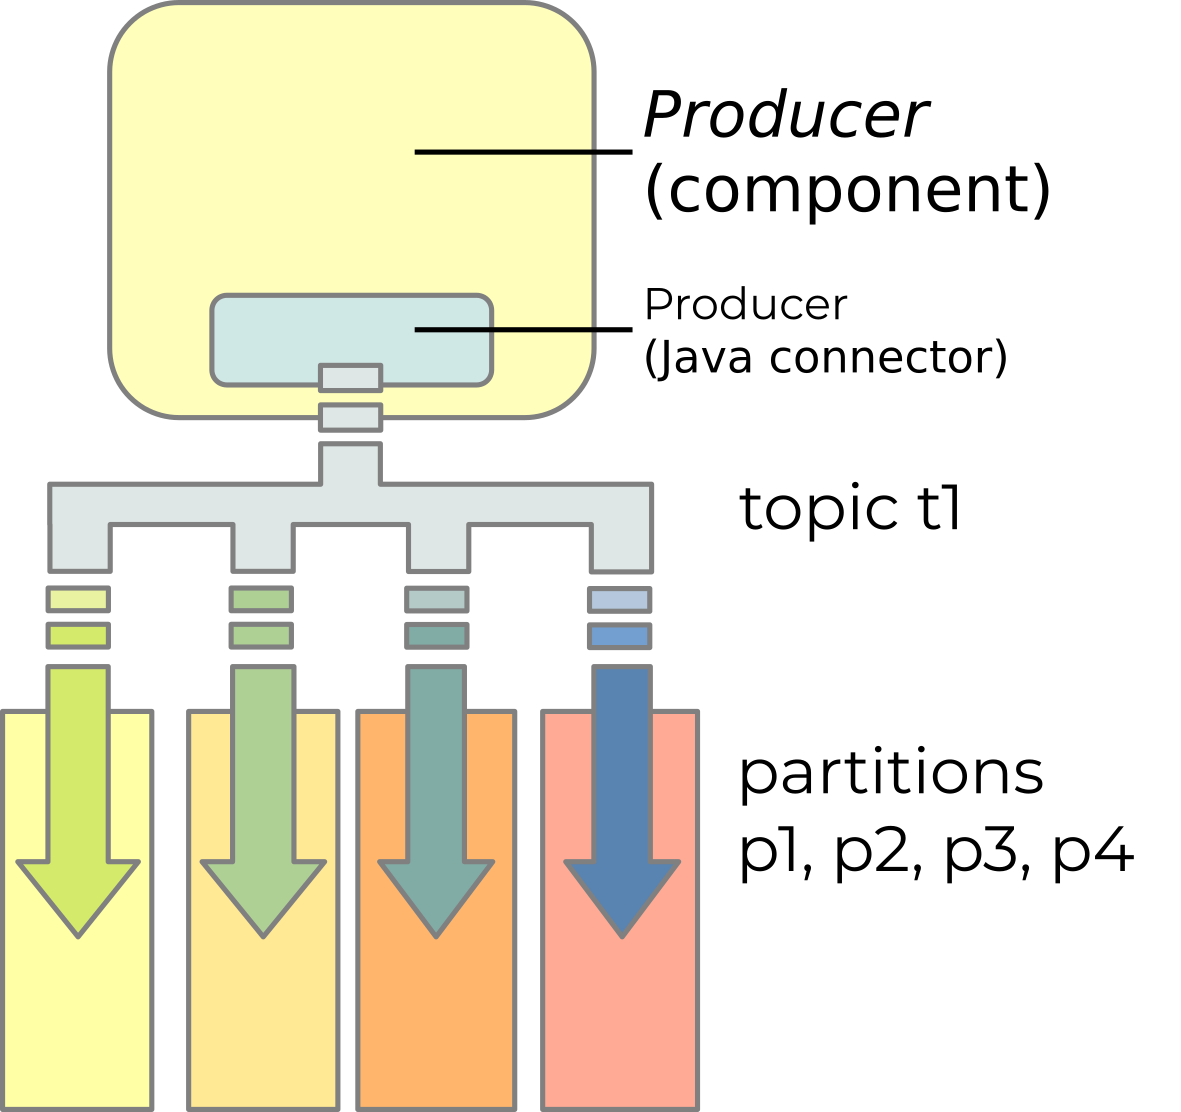
\includegraphics{images/kafka-partitions-01.png}
%\includesvg{images/kafka-partitions-01.svg}
\caption{Client \javaname{Producer} distributes messages to partitions}
\label{fig:kafka-partitions-01}
\end{center}
\end{figure}

\clearpage
The total number of log files is set by the number of partitions multiplied by the replication factor set for that topic.
If a topic has four partitions, and a replication factor of three, then the data will be spread across twelve log files.
If this topic is served by four servers, then each server will be allocated three of the twelve files.

The \javaname{Producer} client connector writes each partition to one server. Replicating the data to the other servers in the cluster is handled internally by server to server transfers.

\begin{figure}[H]
\begin{center}
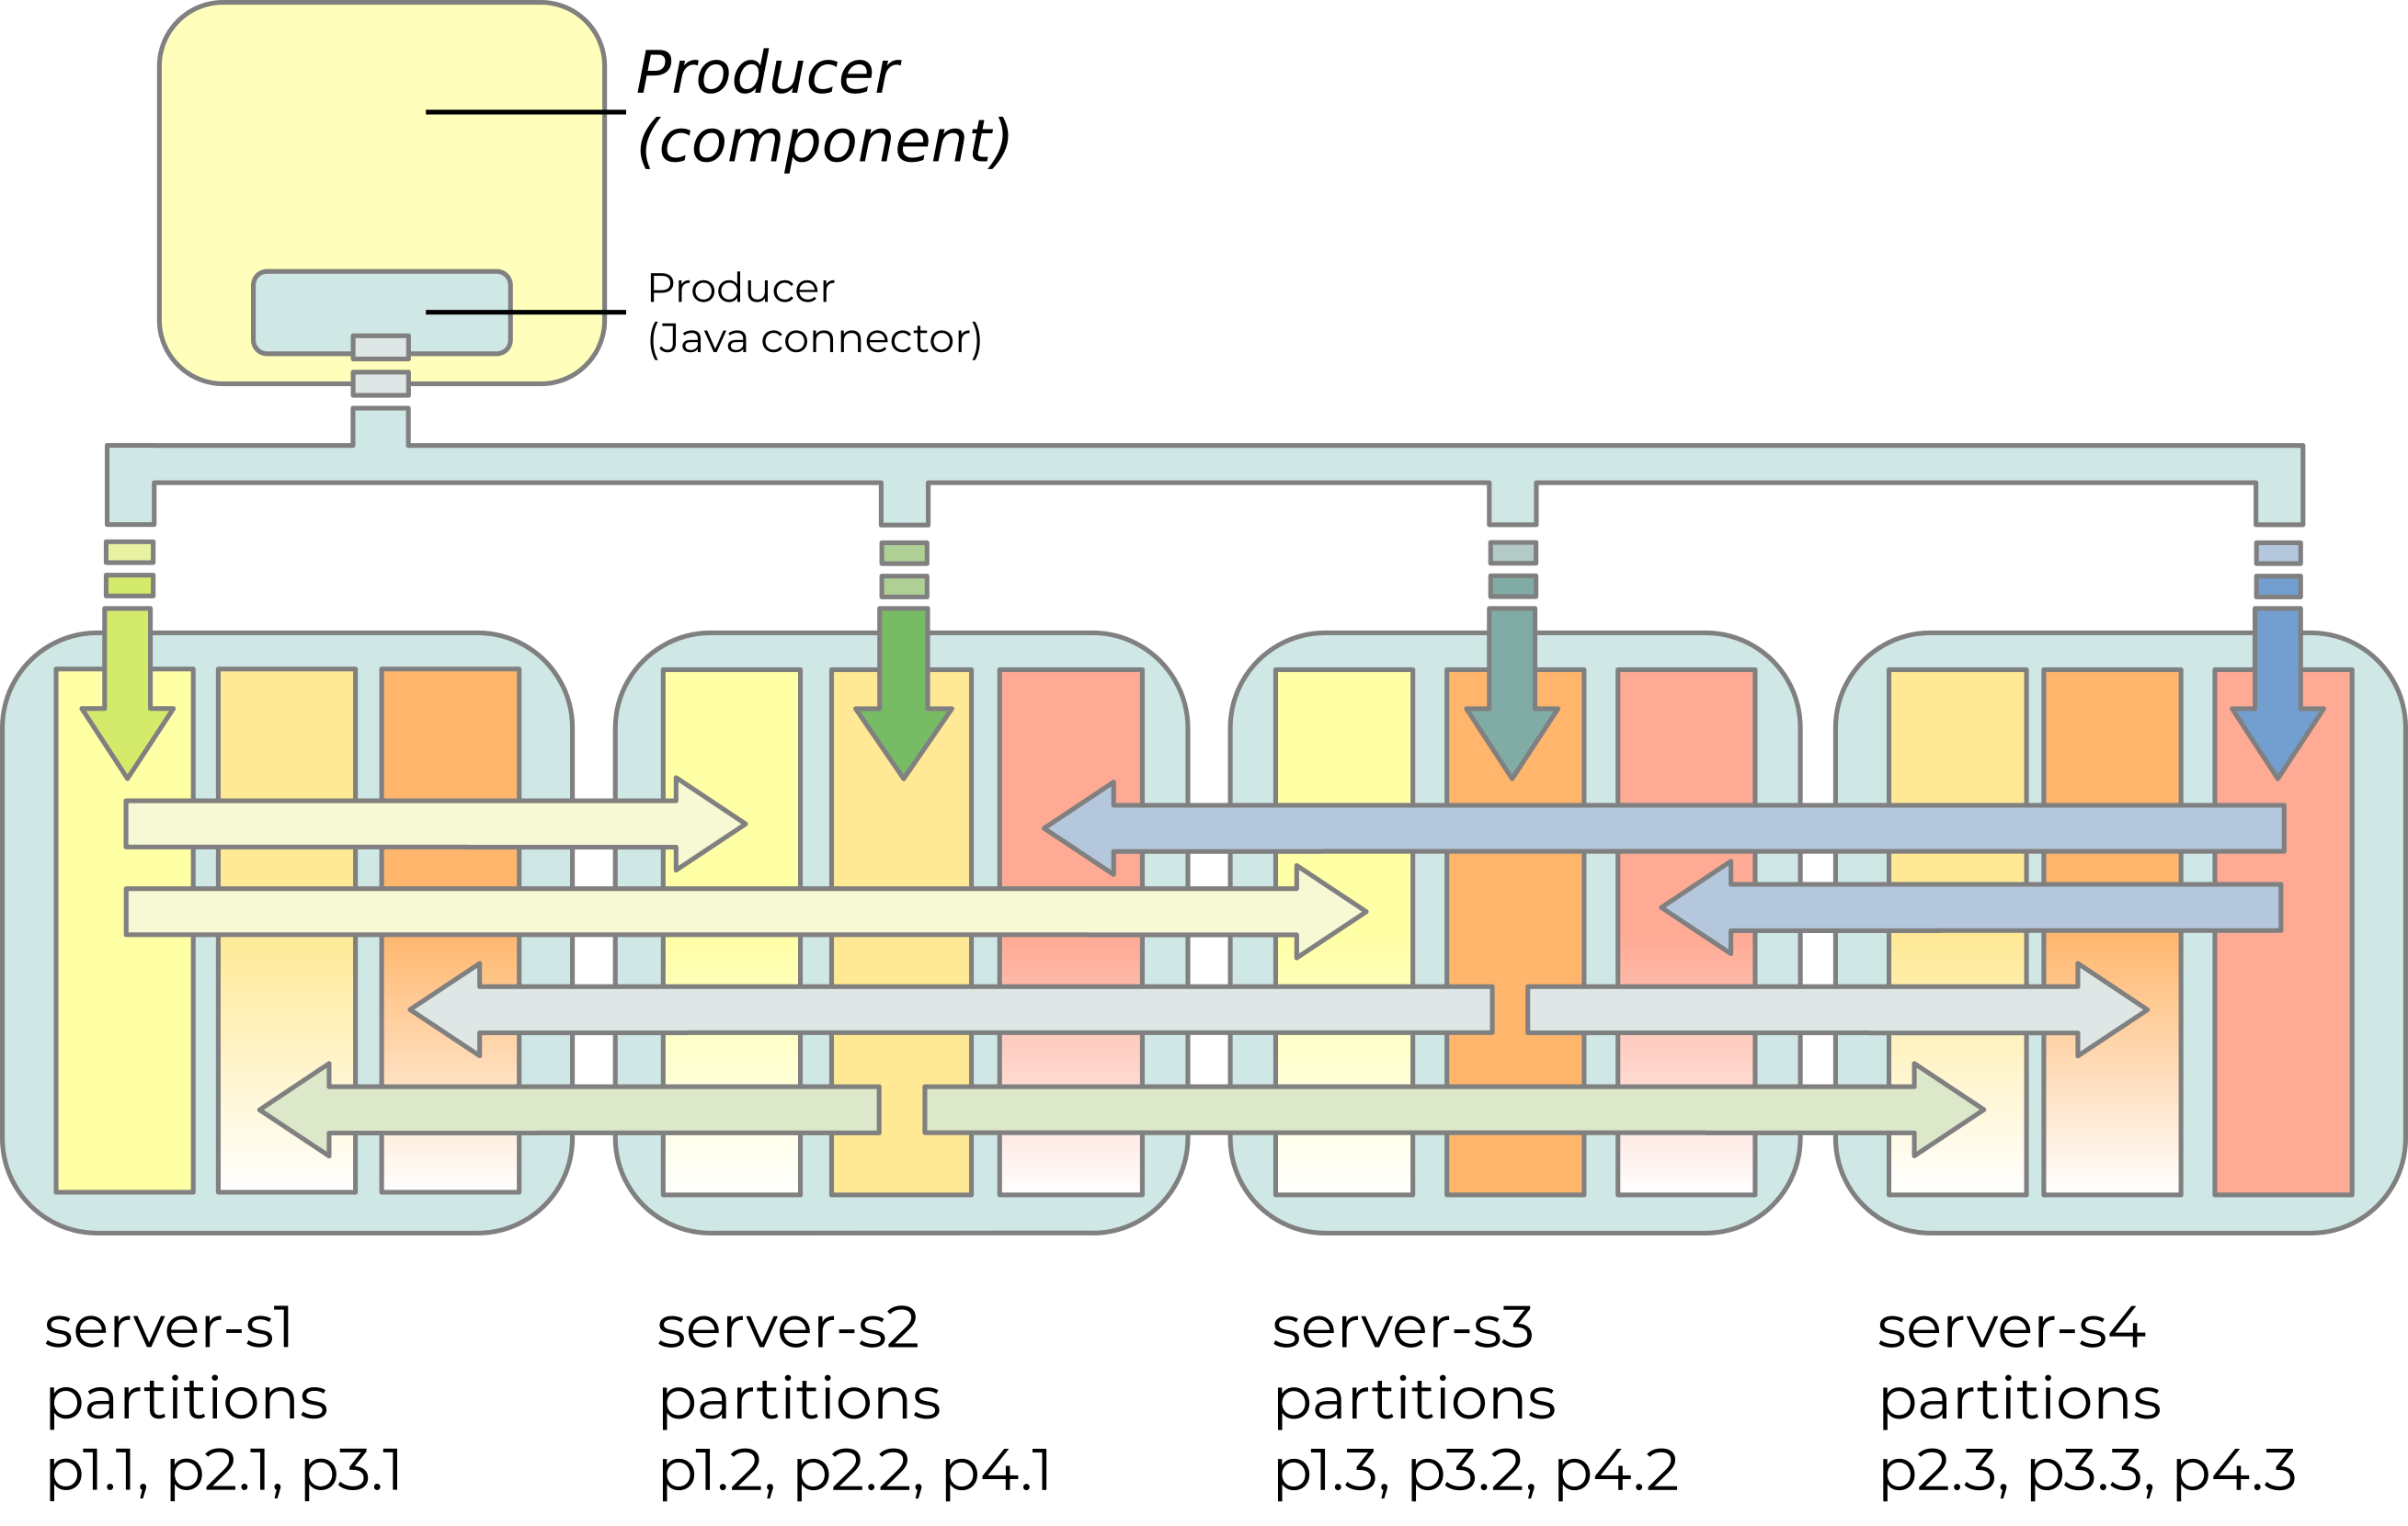
\includegraphics{images/kafka-partitions-03.png}
%\includesvg{images/kafka-partitions-03.svg}
\caption{Client \javaname{Producer} distributes messages to partitions}
\label{fig:kafka-partitions-01}
\end{center}
\end{figure}

\clearpage
I we loose one of the machines, server-s2 for example, the system still has two copies of each of the three partition files that were on server-s2.

\begin{itemize}
    \item partition-p1 is on server-s1 and server-s3
    \item partition-p2 is on server-s1 and server-s4
    \item partition-p4 is on server-s3 and server-s4
\end{itemize}

If we replace server-2 with an empty machine, the three missing log files can be recovered using data from the other servers.

\begin{figure}[H]
\begin{center}
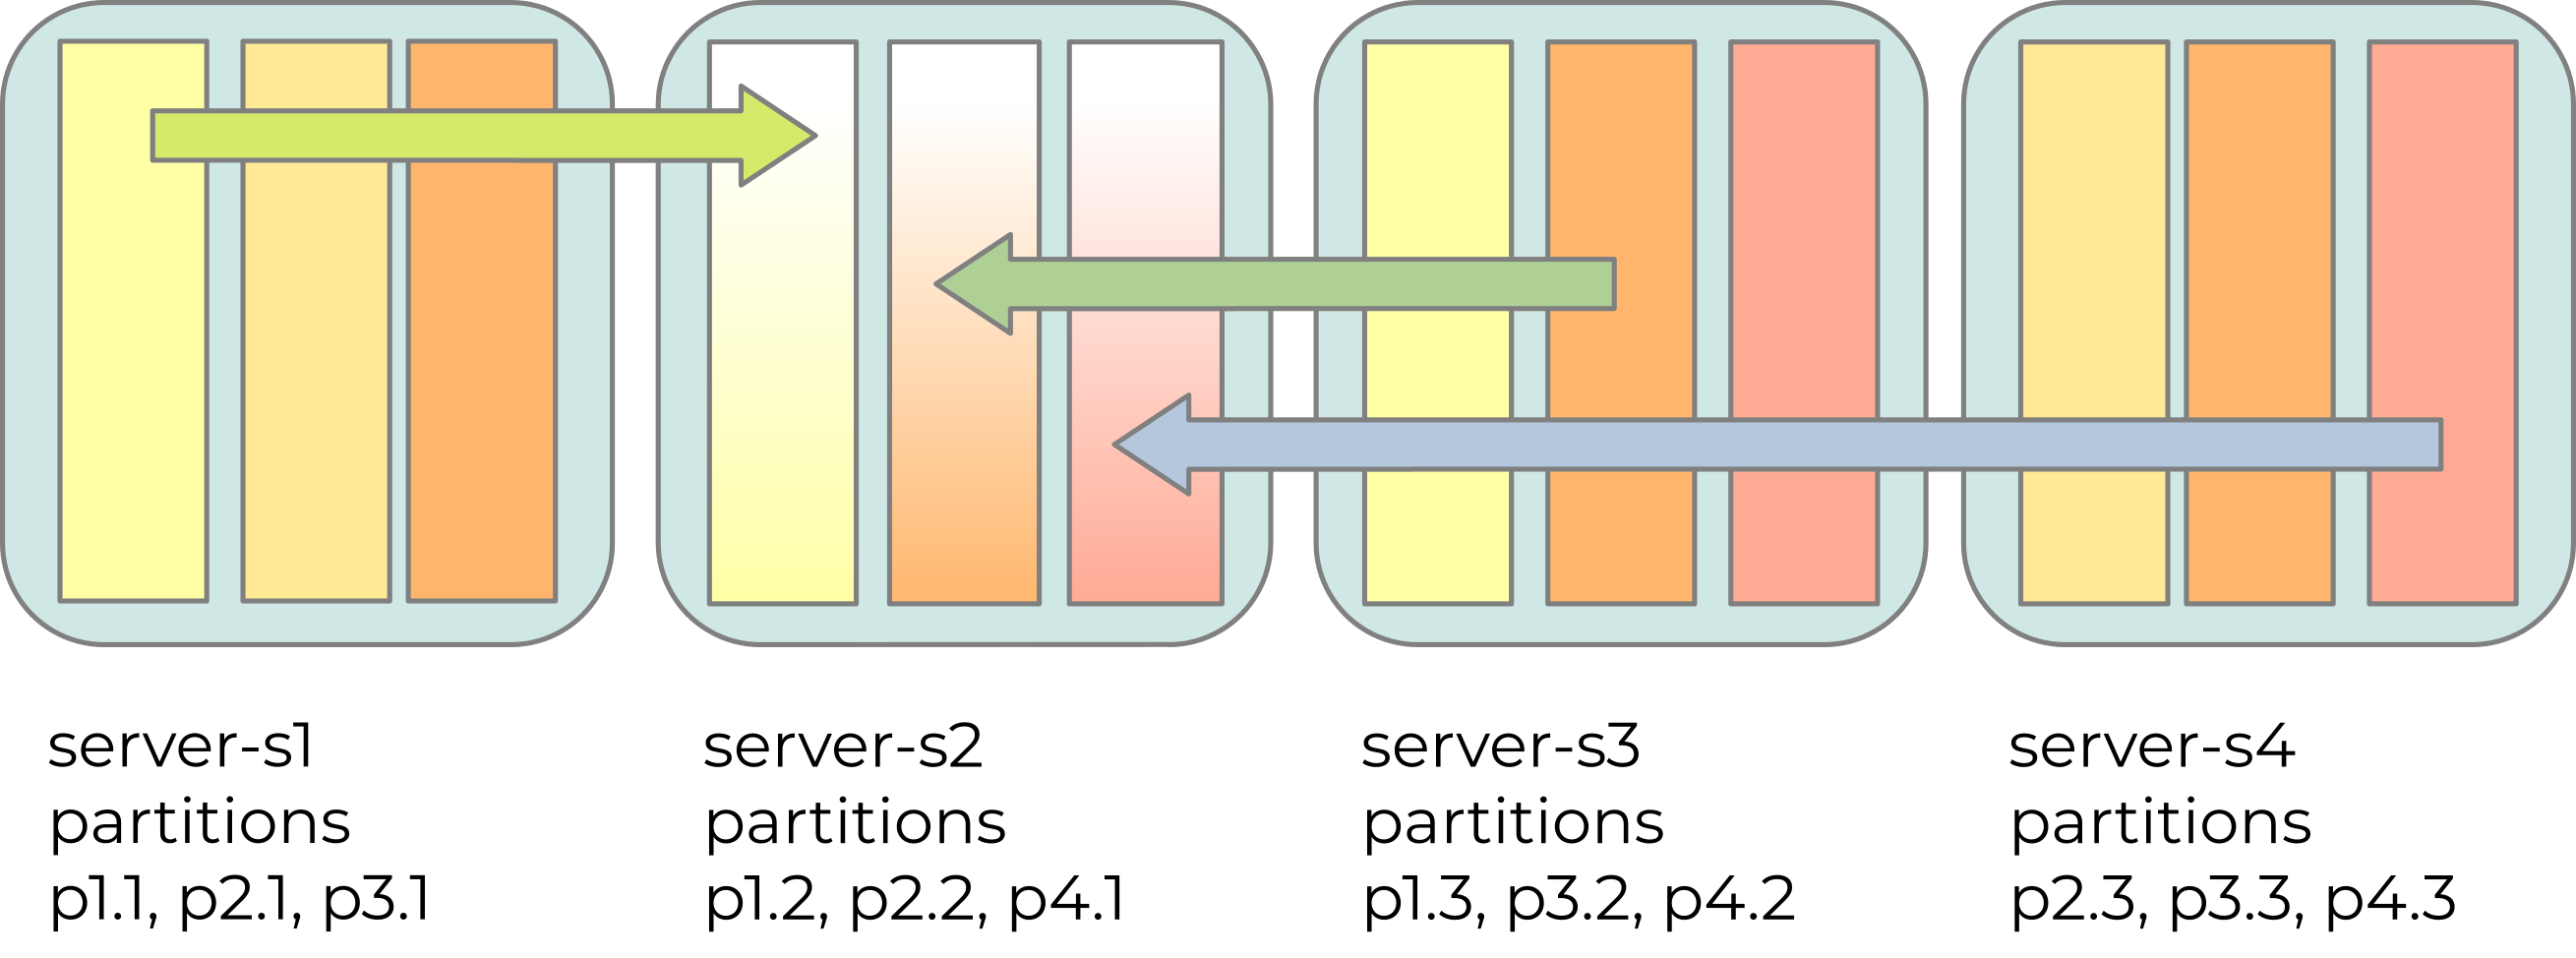
\includegraphics{images/kafka-partitions-04.png}
%\includesvg{images/kafka-partitions-04.svg}
\caption{Missing data recovered from replicas}
\label{fig:kafka-partitions-01}
\end{center}
\end{figure}

\clearpage

\subsection{Kafka partitions}
\label{kafka-partitions}

The partitioning and replication of data is essential to the way that Kafka operates, and provides much of the performance and reliability benefits of Kafka.
However, the same partitioning and duplication can also cause a number of
side effects that we need to be aware of.

One of the issues that needs to be considered for a Kafka deployment is the number of partitions that the data for a topic is split into.

The number of partitions assigned to a topic directly influences
the level of concurrency available to downstream processing nodes.

Spreading data across partitions is not done by the services.
The spread across partitions is performed by the upstream producer that writes
the data to the service.

When a client producer writes data to a service, it first requests
the number of partitions assigned to the topic by querying the
server to request the topic configuration.

If we start with an example configuration of one producer connected to
a set of four servers.

If the topic that the producer is writing to is configured with only three partitions,
then the producer will split the data into blocks and send them to one of three
partitions in turn.

The first block will be sent to partition one on the first server, the second block is sent to
partition two on the second server, and the third block is sent to partition three on the third server.

The fourth block is sent to partition one on the first server,
the fifth to partition two on the second server and the sixth block to partition three on the the third server.

In this simple configuration, with more servers than partitions, the fourth server
does not have any partitions allocated to it.
In reality, the replication factor would normally be greater than one, so internal
replication would spread copies of the data between the four servers, including
the fourth service.
However, to simplify this example we are only tracking the primary copies for
each partition and not the replicas.

If we increase the partition count to four, then the partitions are spread
evenly across all four servers.

With five partitions, then three of the four servers would have one partition each,
and one of the servers would have two partitions.

As the number of partitions increases, the data is spread more evenly across the servers.

With twenty five partitions, three of the four servers would have six
partitions, and one of the servers would have seven partitions.

With one hundred and twenty five partitions, three of the four servers would have thirty one
partitions, and one of the servers would have thirty two partitions.


With data being written into our service, we can now look at
how the data is sent to downstream consumers.

Starting with the first example, three partitions spread across four servers.
If we have a single consumer, then data from all four partitions are sent to the
same consumer.

If we have two consumers, the first consumer would be sent data for one partition,
and the second consumer would be sent data for two partitions.

If we have three consumers, then each consumer handles data from one partion.

If we have four consumers, then three of the consumers each handle data one partion,
and the fourth consumer does not receive any data.

Increasing the number of consumers beyond the number of partitions
results in idle consumers with no data sent to them.

This limits the level of concurrency that the downstream component can be configured with.
With three partitions, then the system will only send data to three consumers.
Adding more consumers running in parallel will not increase the data throughput.

With twenty five partitions, we can add up to twenty five consumers running in parallel,
and each consumer will receive data from one partition.

With one hundred and twenty five partitions, we can add up to hundred and twenty five
consumers running in parallel.

The general rule is configuring a topic to have more partitions spreads the data more
evenly accross the available resources.

This is a dynamic process. If we add more servers to a live cluster, the servers in the cluster
will automatically assign partions to the new joiners, balancing the partitions
and replication between the available resources.

Likewise adding more consumers to a consumer group, the servers will automatically assign
partions to the new joiners, balancing the partitions between the consumers.

If we have twenty five partitions and ten consumers, then five of the consumers will be sent
data from three partitions, and five of the consumers will be sent data from two partitions.

As we add more consumers to the group the servers will dynamically re-allocate
partitions between the consumers.

With eleven consumers, eight consumers will get data from two partitions and
three will get data from three partitions.

This works all the way up to twenty five consumers, each handling data from one partition.

Adding a twenty sixth consumer will not spread the data from a partion between two
consumers. So the twenty sixth consumer will not get any data.

The general rule is splitting the data across more partitions in the service means it can be spread
across more concurrent consumers downstream.
The number of partitions in the service sets the upper limit on the number of concurrent
consumers downstream.
Having more consumers than partitions will result in consumers sitting idle with no data being sent to them.

Note that the number of consumers in these examples equates to the number of concurrent threads.
In terms of data partitioning, a single consumer process with four threads is the same as
four consumers running one thread each.

Talking about a hundred partitions sounds a lot, but consider if we use two of the LSST:UK test bed machines
with 28 cpu cores each, with hyper-threading (https://en.wikipedia.org/wiki/Hyper-threading) enabled,
that gives us a potential (28*2*2) = 112 concurrent threads.
If we want to be able to dynamically add extra processing to the system in response to load, then
adding a third machine would give us 168 threads, and a fourth machine would give us a total of 224
concurrent threads.

In order to be able to scale the system to this level, we would need to allocate enough partitions
to be able to share the data across all 224 threads.

However, there are costs associated with increasing the number of partitions.
The primary cost of splitting the data across a large number of partitions is the amount of resources this consumes on the servers.

If we consider the stage 1 top level FIFO buffer, there are likley to be several logical client processes
receiving data from the same buffer topic.
We may have three or four processors consuming data from the stream and performing catalog \crossmatch or
watch list triggers.
We may have a couple of processors consuming data from the stream and extracting the thumbnail images or light curves, and we may have a couple of processors consuming data from the stream and archiving it as Avro or Parquet files for downstream analysis tools.

The way that Kafka is able to handle multiple processes consuming data at different rates is by appending the data to flat log files, one for each partition, and maintaining a separate offset pointer for each consumer.

When a group of consumers subscribe to a topic, the servers assigns the available partitions to the members of the group, storing an offset pointer for each consumer for each partiton it is allocated.

When a consumer requests a block of data, the server loads the next available block from one of the partions allocated to that consumer using the offset pointer for that consumer on that partition.
The server loads the data into a buffer in memory, sends it to the consumer and waits for an acknowledgment.
When it receives an acknowledgment from the consumer, the server increments the offset pointer for that consumer on that partition and then loads the next block of data to send

If we allocate separate consumer processes to each watch list, \crossmatch, filter or characterization process, then our stage 1 FIFO buffer may have a hundred processes subscribed to read data from the topic.

Each of these logical processes consists of a group of concurrent consumer processes running on one or more of the worker nodes.

Irrespective of how many concurrent threads they are running, each consumer group will need to allocate
a consumer connection to each partition.

A hundred consumer groups means a hundred connections to each partition.

If we distribute our data across 224 partitions, then our server machine has to handle 224 partitions, with 100 connections to each partition, each connection needing a buffer for the data, an offset counter and an open file descriptor to read the data.

The second cost of splitting the data across a large number of partitions is the amount of resources this consumes on the client.
If we have 224 partitions and 224 consumer threads, then in theory each consumer should only need to handle data for one partition, or 1/224 of the data.

However, the way that the connection process works means there is a race condition at the start of the process.
The first consumer to subscribe to a topic is allocated all of the partitions for that topic.
When the second consumer subscribes, half of the partitions are re-allocated to the new joiner.
When the third consumer subscribes, a third of the partitions are re-allocated to the new joiner, and so on.

The problem is that at the start of the process when there are only a few consumers subscribed to the topic,
they have to share all of the partitions between them. Worst case is the short period when only one
consumer is subscribed, it has to handle network connections and data buffers for all 244 topics.

\subsection{Kafka  archive}
\label{kafka-archive}


\printbibliography

\end{document}
